%%%%%%%%%%%%%%%%%%%%%%%%%%%%%%%%%%%%%%%%%%%%%%%%%%%%%%%%%%%%%%%%%%%%%%%%%%%%%%%%%%
\begin{frame}[fragile]\frametitle{}
\begin{center}
{\Large Descriptive Statistics}
\end{center}
\end{frame}


%%%%%%%%%%%%%%%%%%%%%%%%%%%%%%%%%%%%%%%%%%%%%%%%%%%%%%%%%%%
\begin{frame}[fragile]\frametitle{Descriptive Statistics}
\begin{itemize}
\item Describes the data characteristics
\item To make sense of the data
\item To make rational decisions
\item E.g. Demographics, clinical data.
\item Measures of Central Tendencies
\item Measures of Variability
\item Measures of Shape
\end{itemize}
\end{frame}

%%%%%%%%%%%%%%%%%%%%%%%%%%%%%%%%%%%%%%%%%%%%%%%%%%%%%%%%%%%
\begin{frame}[fragile]\frametitle{Why Descriptive Statistics?}
\begin{itemize}
\item Population: the whole
\item Sample: small subset of the population
\item Gauging Population by examining traits of Sample.
\item Example Question: Finding height of Americans?
\item Not going to measure everyone height, but that in a {\bf representative} sample.
\item Example: Election sampling?
\end{itemize}
\end{frame}



%%%%%%%%%%%%%%%%%%%%%%%%%%%%%%%%%%%%%%%%%%%%%%%%%%%%%%%%%%%
\begin{frame}[fragile]\frametitle{Why Descriptive Statistics?}
\begin{itemize}
\item To check the accuracy and precision of the process
\item To reduce variability and improve process capability
\item To know the truth about the real world
\end{itemize}
\end{frame}


%%%%%%%%%%%%%%%%%%%%%%%%%%%%%%%%%%%%%%%%%%%%%%%%%%%%%%%%%%%%%%%%%%%%%%%%%%%%%%%%%%
\begin{frame}[fragile]\frametitle{}
\begin{center}
{\Large Basic Terms}
\end{center}
\end{frame}

%%%%%%%%%%%%%%%%%%%%%%%%%%%%%%%%%%%%%%%%%%%%%%%%%%%%%%%%%%%%%%%%%%%%%%%%
\begin{frame}[fragile]\frametitle{Histogram}

\begin{columns}
    \begin{column}[T]{0.6\linewidth}
Example
	\begin{itemize}
	\item Say, we are measuring height of people.
	\item Plotting them on X axis.
	\item The dots would look very crowded where there are many close or repetitive observations.
	\item Some dots get hidden.
	\item We can improve the visualization, by plotting frequency (number of occurrences) on Y axis.
	\item But in case of contiguous variable, like, exact measurements are rare. So we `bin' them and measure occurrences.
	\item Thats Histogram.
	\end{itemize}

    \end{column}
    \begin{column}[T]{0.4\linewidth}
      \begin{center}
      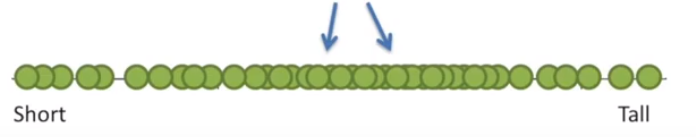
\includegraphics[width=\linewidth,keepaspectratio]{statq1}
	  
	  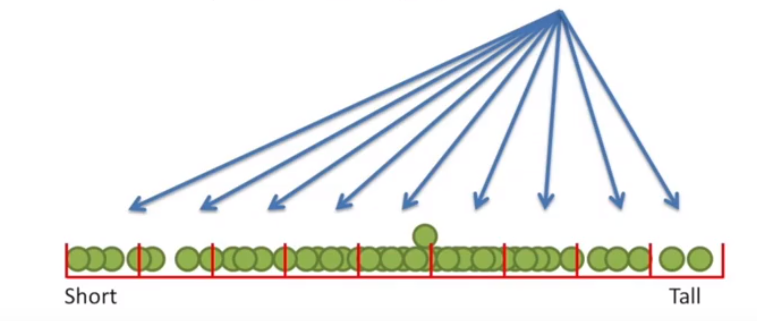
\includegraphics[width=\linewidth,keepaspectratio]{statq2}
	  
	  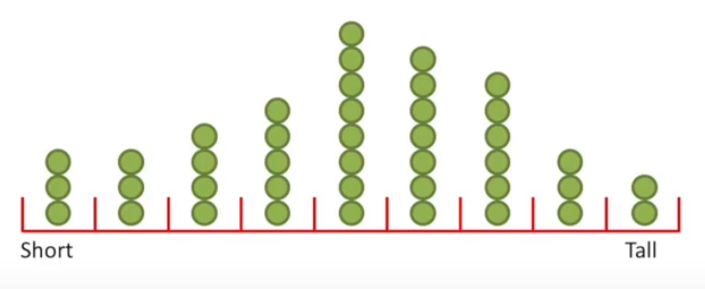
\includegraphics[width=\linewidth,keepaspectratio]{statq3}	  
	  	\end{center}
    \end{column}

  \end{columns}
  

\tiny{(Ref: StatQuest: What is a Histogram? - Josh Starmer )}
\end{frame}

%%%%%%%%%%%%%%%%%%%%%%%%%%%%%%%%%%%%%%%%%%%%%%%%%%%%%%%%%%%%%%%%%%%%%%%%
\begin{frame}[fragile]\frametitle{Histogram}

\begin{columns}
    \begin{column}[T]{0.6\linewidth}

	\begin{itemize}
	\item Histogram can be used to predict probability of getting (future) measurements.
	\item Getting measurement (as shown in the box) in the middle region is more likely.
	\item Measurements at both the ends are rare.
	\item We can approximate this histogram of observations by a `distribution'.
	\item Looks like `Normal' distribution, or a bell-curve
	\end{itemize}

    \end{column}
    \begin{column}[T]{0.4\linewidth}
      \begin{center}
      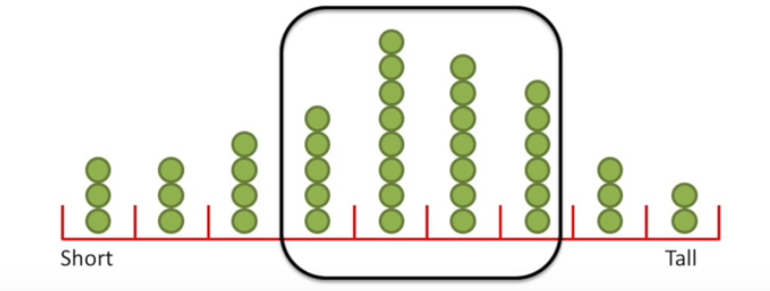
\includegraphics[width=\linewidth,keepaspectratio]{statq4}
	  
	  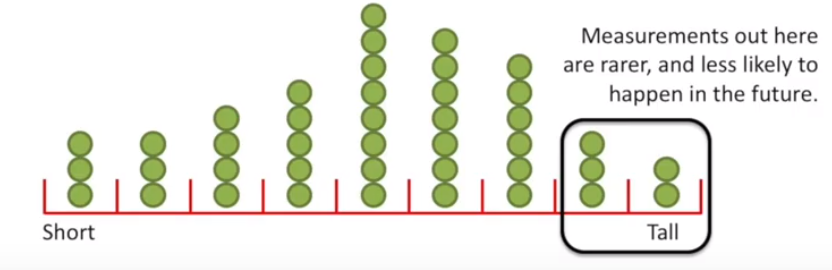
\includegraphics[width=\linewidth,keepaspectratio]{statq5}
	  
	  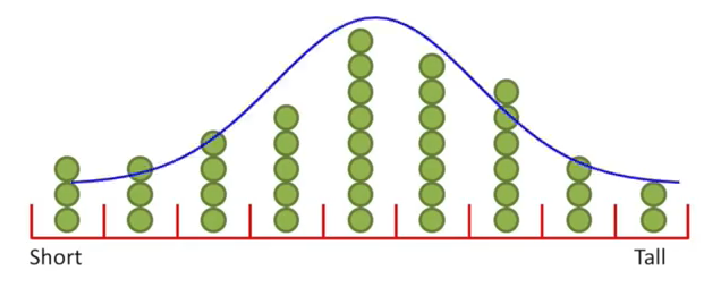
\includegraphics[width=\linewidth,keepaspectratio]{statq6}	  
	  	\end{center}
    \end{column}

  \end{columns}
  

\tiny{(Ref: StatQuest: What is a Histogram? - Josh Starmer )}
\end{frame}

%%%%%%%%%%%%%%%%%%%%%%%%%%%%%%%%%%%%%%%%%%%%%%%%%%%%%%%%%%%%%%%%%%%%%%%%
\begin{frame}[fragile]\frametitle{Histogram}

\begin{columns}
    \begin{column}[T]{0.6\linewidth}

	\begin{itemize}
	\item If the frequency of measurements seem decreasing, it may be an exponential distribution.
	\item Binning criterion is critical. They can not be too narrow or too wide.
	\item Try different bin widths/formulas to plot a histogram.
	\end{itemize}

    \end{column}
    \begin{column}[T]{0.4\linewidth}
      \begin{center}
      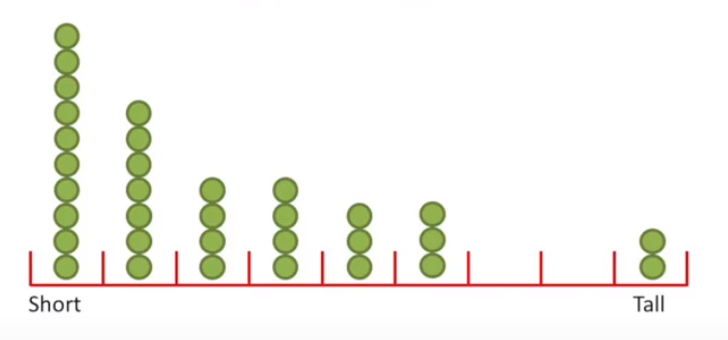
\includegraphics[width=\linewidth,keepaspectratio]{statq7}
	  
	  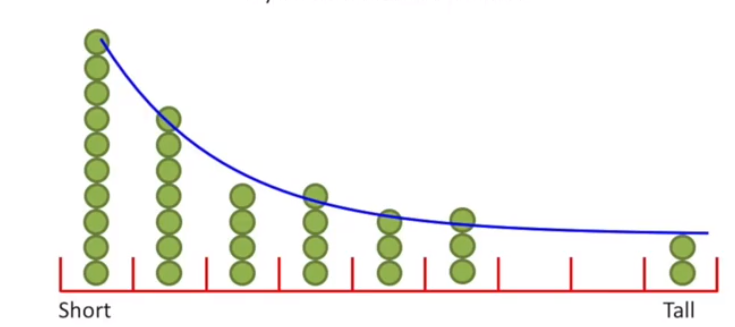
\includegraphics[width=\linewidth,keepaspectratio]{statq8}
	  
	  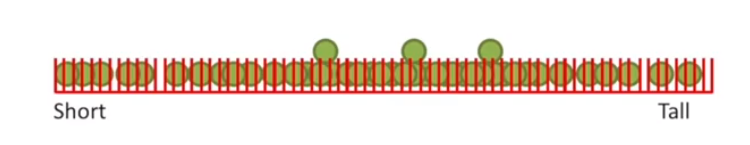
\includegraphics[width=\linewidth,keepaspectratio]{statq9}	  
	  	\end{center}
    \end{column}

  \end{columns}
  

\tiny{(Ref: StatQuest: What is a Histogram? - Josh Starmer )}
\end{frame}


%%%%%%%%%%%%%%%%%%%%%%%%%%%%%%%%%%%%%%%%%%%%%%%%%%%%%%%%%%%%%%%%%%%%%%%%%%%%%%%%%%
\begin{frame}[fragile]\frametitle{}
\begin{center}
{\Large Descriptive Statistics Example}
\end{center}
\end{frame}


%%%%%%%%%%%%%%%%%%%%%%%%%%%%%%%%%%%%%%%%%%%%%%%%%%%%%%%%%%%
\begin{frame}[fragile]\frametitle{Descriptive Statistics}
\begin{itemize}
\item Describes features of data sets using numbers
\item Individual row: Data
\item Full table: Dataset
\item Purpose: Answer questions.
\end{itemize}
\begin{center}
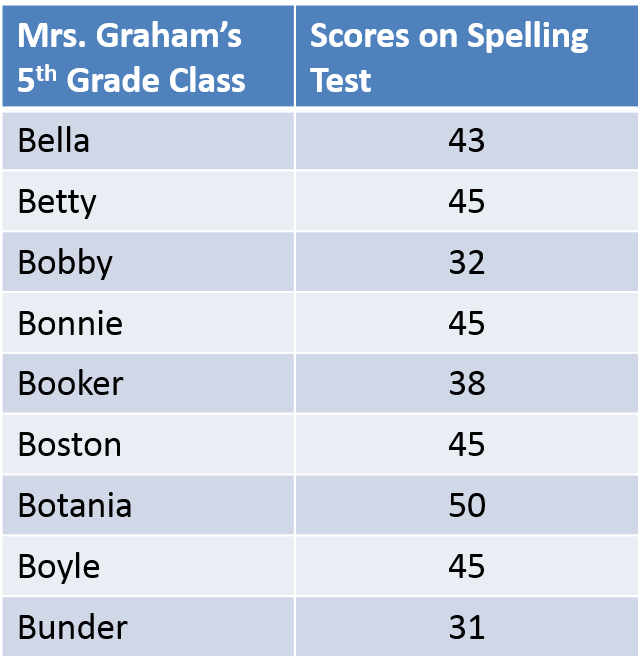
\includegraphics[width=0.35\linewidth,keepaspectratio]{da1}
\end{center}
\end{frame}

%%%%%%%%%%%%%%%%%%%%%%%%%%%%%%%%%%%%%%%%%%%%%%%%%%%%%%%%%%%
\begin{frame}[fragile]\frametitle{Questions}
\begin{center}
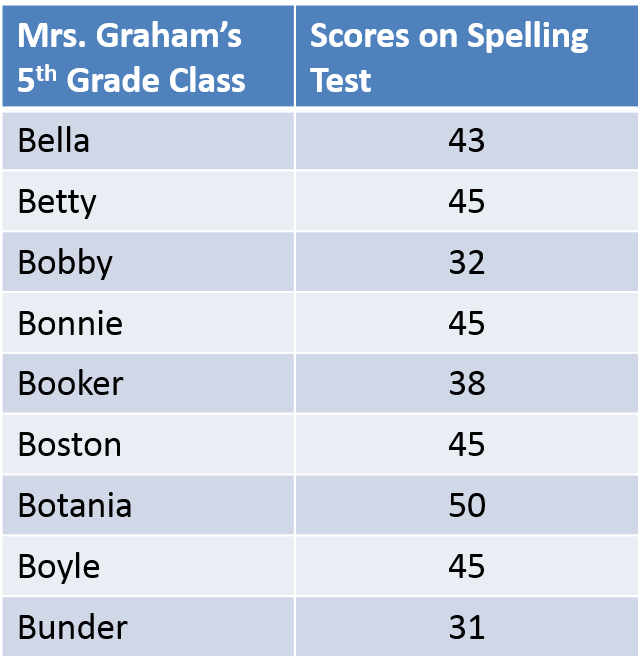
\includegraphics[width=0.35\linewidth,keepaspectratio]{da1}
\end{center}
\begin{itemize}
\item What is Bobby's score?
\item Out of? (Total \# entries)
\item Highest/Lowest scores?
\end{itemize}
\end{frame}

%%%%%%%%%%%%%%%%%%%%%%%%%%%%%%%%%%%%%%%%%%%%%%%%%%%%%%%%%%%
\begin{frame}[fragile]\frametitle{Questions}
\begin{center}
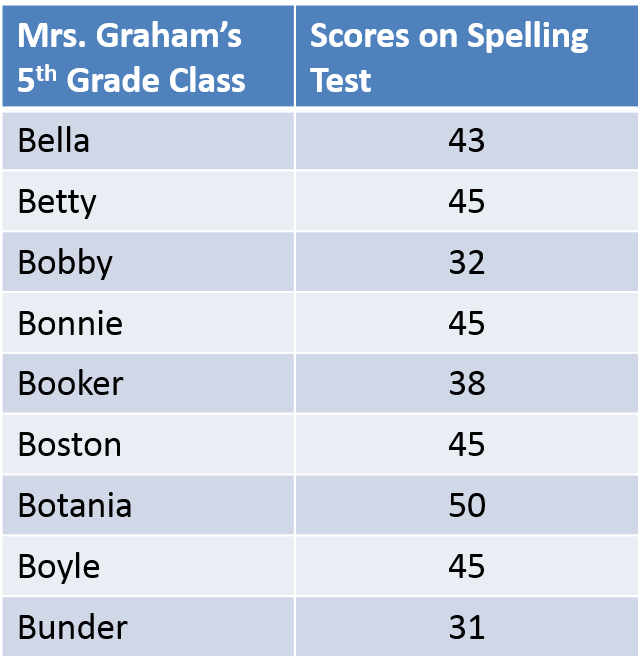
\includegraphics[width=0.35\linewidth,keepaspectratio]{da1}
\end{center}
\begin{itemize}
\item Class average?
\item Most Common/frequent Score?
\item Any other questions?
\end{itemize}
\end{frame}

%%%%%%%%%%%%%%%%%%%%%%%%%%%%%%%%%%%%%%%%%%%%%%%%%%%%%%%%%%%
\begin{frame}[fragile]\frametitle{Numerical Measures}
\begin{itemize}
\item Highest to Lowest Score: RANGE
\item Most Common Score: MODE
\item Average Score: MEAN
\item Any other measures?
\end{itemize}
\end{frame}

%%%%%%%%%%%%%%%%%%%%%%%%%%%%%%%%%%%%%%%%%%%%%%%%%%%%%%%%%%%
\begin{frame}[fragile]\frametitle{Descriptive Statistics}
\begin{itemize}
\item Examines ALL data (not sample)
\item Cannot generalize to other datasets
\end{itemize}
\end{frame}

%%%%%%%%%%%%%%%%%%%%%%%%%%%%%%%%%%%%%%%%%%%%%%%%%%%%%%%%%%%%%%%%%%%%%%%%%%%%%%%%%%
\begin{frame}[fragile]\frametitle{}
\begin{center}
{\Large Descriptive Statistics Example}
\end{center}
\end{frame}


%%%%%%%%%%%%%%%%%%%%%%%%%%%%%%%%%%%%%%%%%%%%%%%%%%%
\begin{frame}[fragile] \frametitle{Descriptive Tasks}

\adjustbox{valign=t}{
\begin{minipage}{0.45\linewidth}
\begin{center}
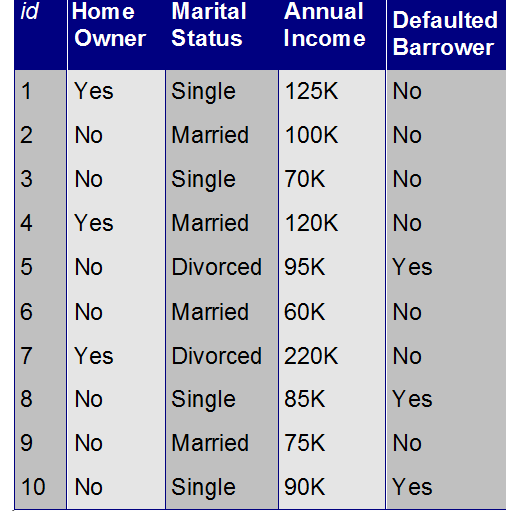
\includegraphics[width=\linewidth,keepaspectratio]{descriptivetable}
\end{center}
\end{minipage}
}
\hfill
\adjustbox{valign=t}{
\begin{minipage}{0.45\linewidth}
\begin{itemize}
\item Objective: Derive patterns, summarize underlying relationships
\item More exploratory of current state
\end{itemize}
\end{minipage}
}

\end{frame}



%%%%%%%%%%%%%%%%%%%%%%%%%%%%%%%%%%%%%%%%%%%%%%%%%%%%%%%%%%
\begin{frame}[fragile]\frametitle{Data Example}	
\begin{center}
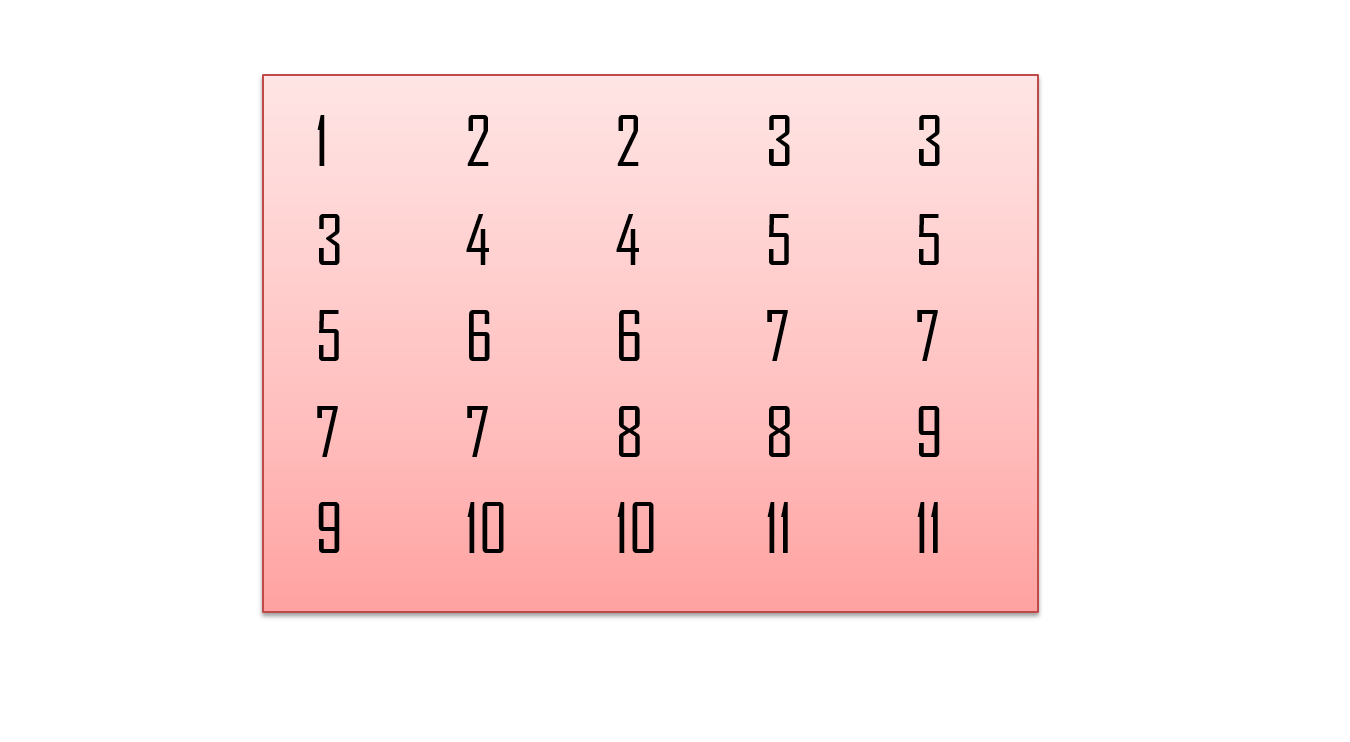
\includegraphics[width=0.8\linewidth,keepaspectratio]{da2}
\end{center}
What sense it makes?
Any pattern?


%\code{Store as list of integers}
\end{frame}

%%%%%%%%%%%%%%%%%%%%%%%%%%%%%%%%%%%%%%%%%%%%%%%%%%%%%%%%%%
\begin{frame}[fragile]\frametitle{Visualize}	
\begin{center}
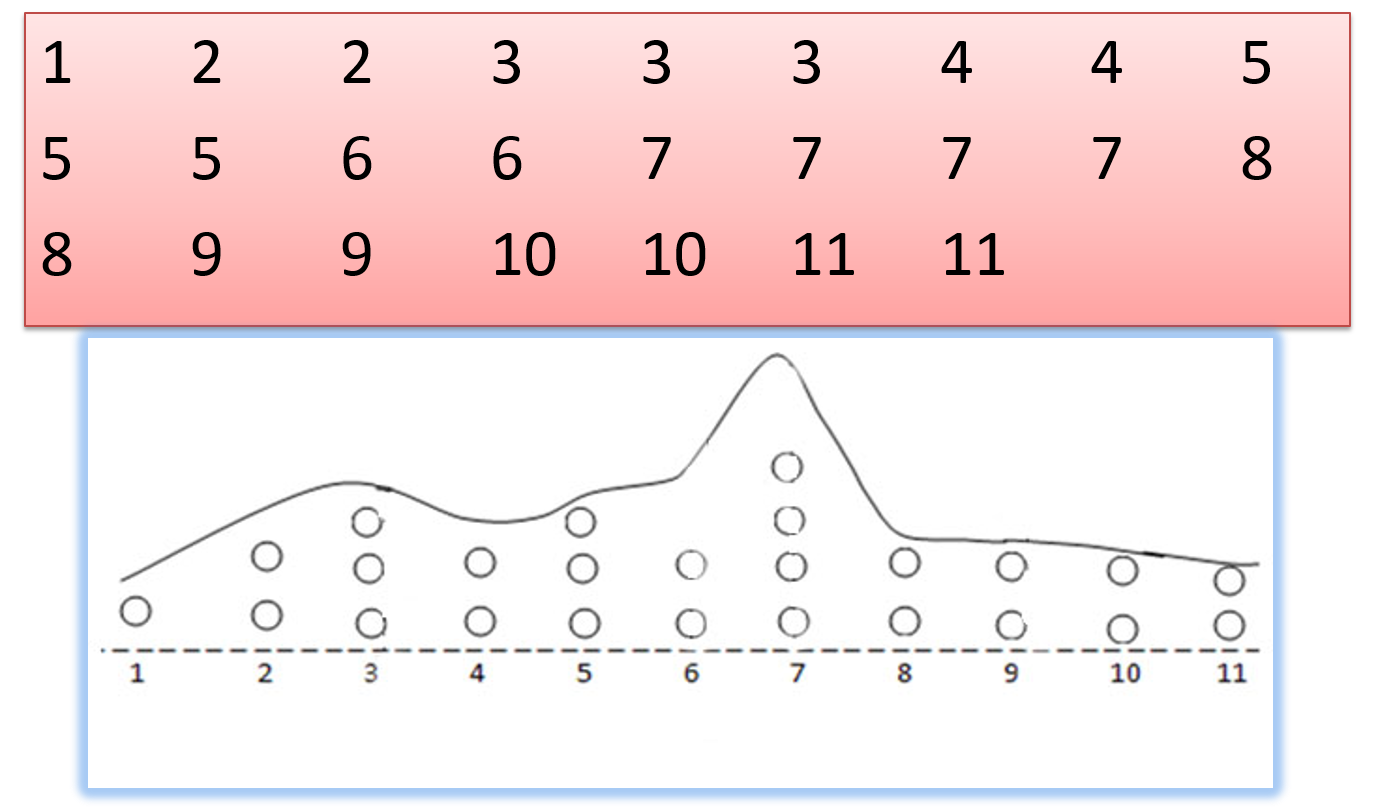
\includegraphics[width=0.8\linewidth,keepaspectratio]{da3}
\end{center}
Makes sense?


%\code{Plot the data points, not the curve}
\end{frame}

%%%%%%%%%%%%%%%%%%%%%%%%%%%%%%%%%%%%%%%%%%%%%%%%%%%%%%%%%%
\begin{frame}[fragile]\frametitle{The Shape of The Distribution}	
Better to see
\begin{center}
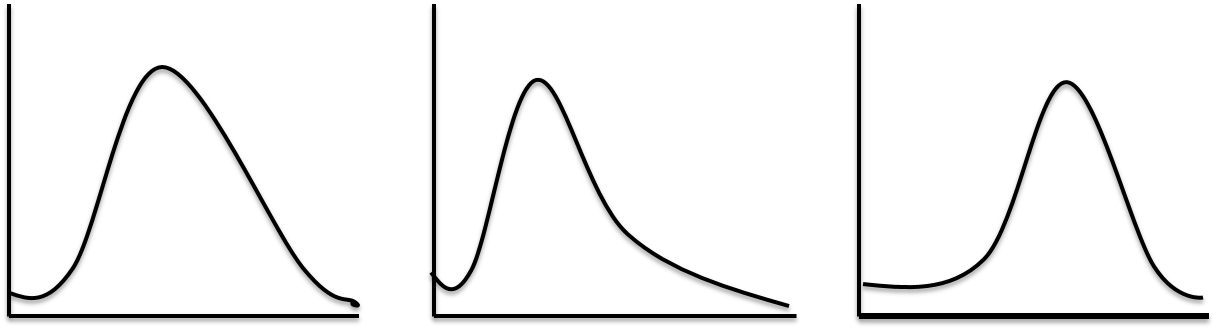
\includegraphics[width=0.8\linewidth,keepaspectratio]{da4}
\end{center}
Symmetric? Skewed right/left?
%\code{Plot the curve}
\end{frame}

%%%%%%%%%%%%%%%%%%%%%%%%%%%%%%%%%%%%%%%%%%%%%%%%%%%%%%%%%%%%%%%%%%%%%%%%%%%%%%%%%%
\begin{frame}[fragile]\frametitle{}
\begin{center}
{\Large Describing Data}
\end{center}
\end{frame}

%%%%%%%%%%%%%%%%%%%%%%%%%%%%%%%%%%%%%%%%%%%%%%%%%%%%%%%%%%
\begin{frame}[fragile]\frametitle{Describing Data}
\begin{itemize}
\item Univariate Analysis: Statistical moments (based on degree)
\begin{itemize}
\item 1st degree: Central tendency: mean, median, mode
\item 2nd degree: Standard Deviation: how wide data is around mean
\item 3rd degree: Skewness: Asymmetric around mean
\item 4th degree: Kurtosis: shape of skewness.
\end{itemize}
\item BiVariate Analysis: covariance, correlation
\item MultiVariate Analysis
\end{itemize}
\end{frame}


%%%%%%%%%%%%%%%%%%%%%%%%%%%%%%%%%%%%%%%%%%%%%%%%%%%%%%%%%%%
\begin{frame}[fragile]\frametitle{Univariate Analysis}
\begin{itemize}
\item Measure of Central Tendency
\item Measure of Spread
\item Measure of Asymmetry
\item Measure of Skewness
\end{itemize}
\end{frame}


%%%%%%%%%%%%%%%%%%%%%%%%%%%%%%%%%%%%%%%%%%%%%%%%%%%%%%%%%%%
%\begin{frame}[fragile]\frametitle{Frequency}	
%$ frequency(v_i) = \frac{Objects\_with\_Attribute\_v_i}{n}$
%\begin{center}
%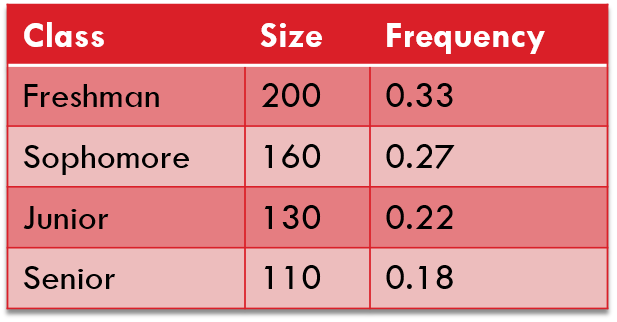
\includegraphics[width=0.8\linewidth,keepaspectratio]{frequency}
%\end{center}
%Often used with categorical values.
%\end{frame}
%

%%%%%%%%%%%%%%%%%%%%%%%%%%%%%%%%%%%%%%%%%%%%%%%%%%%%%%%%%%%%%%%%%%%%%%%%%%%%%%%%%%
\begin{frame}[fragile]\frametitle{}
\begin{center}
{\Large Measure of Central Tendency}
\end{center}
\end{frame}

%%%%%%%%%%%%%%%%%%%%%%%%%%%%%%%%%%%%%%%%%%%%%%%%%%%%%%%%%%
\begin{frame}[fragile]\frametitle{Mean}	
\begin{itemize}
\item Measure the ``location'' of a set of values
\item Mean is a very, very common measurement
\item But is sensitive to outliers
\end{itemize}
$mean(x) = \bar{x} = 1/n \sum x_i$
%\code{Use `for' loop to calculate}
\end{frame}

%%%%%%%%%%%%%%%%%%%%%%%%%%%%%%%%%%%%%%%%%%%%%%%%%%%%%%%%%%
\begin{frame}[fragile]\frametitle{Mean}	
\begin{center}
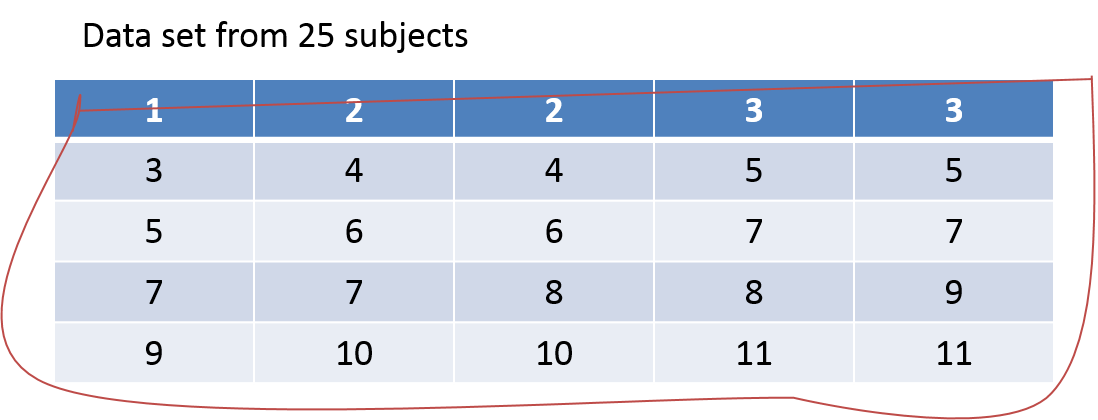
\includegraphics[width=\linewidth,keepaspectratio]{da5}
\end{center}
Sum = 153

Mean = 153/25 = 6.12
\end{frame}

%%%%%%%%%%%%%%%%%%%%%%%%%%%%%%%%%%%%%%%%%%%%%%%%%%%%%%%%%%
\begin{frame}[fragile]\frametitle{Outliers}	
\begin{itemize}
\item Extreme data point
\item May affect calculations
\item  Can occur in any given data set and in any distribution
\item  May indicate an experimental error or incorrect recording of data
\end{itemize}
\begin{center}
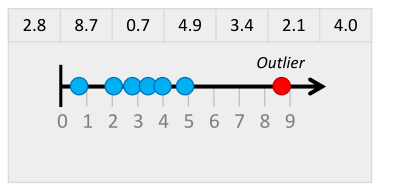
\includegraphics[width=0.6\linewidth,keepaspectratio]{da15}
\end{center}
\end{frame}


%%%%%%%%%%%%%%%%%%%%%%%%%%%%%%%%%%%%%%%%%%%%%%%%%%%%%%%%%%%%%%%%%%%%%%%%
\begin{frame}[fragile]\frametitle{Mean}
Implement mean
\begin{lstlisting}
def mean(datalist):
	:
	return m

lst = [9,3,7,2,7,10,23,44,12,42,19,11,22,5,3,4,3,21,3]
result = mean(lst)
print("Mean : {}".format(result))
\end{lstlisting}
Result?
\end{frame}

%%%%%%%%%%%%%%%%%%%%%%%%%%%%%%%%%%%%%%%%%%%%%%%%%%%%%%%%%%
\begin{frame}[fragile]\frametitle{Mean}
\begin{lstlisting}
def mean(datalist):
	total = 0
	m = 0
	for item in datalist:
		total += item
	m = total / float(len(datalist))
	return m
\end{lstlisting}
Mean : 13.157894736842104
\end{frame}

%%%%%%%%%%%%%%%%%%%%%%%%%%%%%%%%%%%%%%%%%%%%%%%%%%%%%%%%%%
\begin{frame}[fragile]\frametitle{Median}	
\begin{itemize}
\item Commonly used instead of mean if outliers are present
\item Median is the middle value 
\item if odd number of values are present; average of the two middle values if even number of values
\item Not easily affected by outliers (extreme values). 
\item Always exists and unique.
\end{itemize}
$median(x) = x_{r=1} for \quad odd, 1/2(x_r + x_{r+1}) for \quad even$
%\code{Cater to both odd/even case}
\end{frame}


%%%%%%%%%%%%%%%%%%%%%%%%%%%%%%%%%%%%%%%%%%%%%%%%%%%%%%%%%%
\begin{frame}[fragile]\frametitle{Median}	
\begin{center}
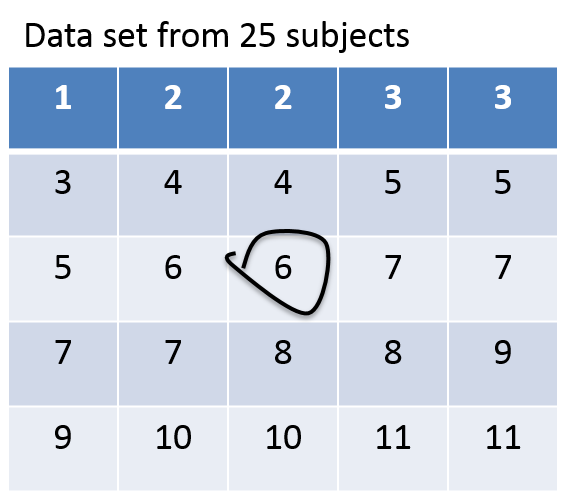
\includegraphics[width=0.5\linewidth,keepaspectratio]{da6}
\end{center}
Median = 6

Medians are less reliable: medians of samples drawn from same population vary more widely than sample means.
%\code{Calculate and verify the answer}
\end{frame}


%%%%%%%%%%%%%%%%%%%%%%%%%%%%%%%%%%%%%%%%%%%%%%%%%%%%%%%%%%%%%%%%%%%%%%%%
\begin{frame}[fragile]\frametitle{Median}
Implement median
\begin{lstlisting}
def median(datalist):
	:
	return m

lst = [9,3,7,2,7,10,23,44,12,42,19,11,22,5,3,4,3,21,3]
result = median(lst)
print("Median : {}".format(result))
\end{lstlisting}
Result?
\end{frame}

%%%%%%%%%%%%%%%%%%%%%%%%%%%%%%%%%%%%%%%%%%%%%%%%%%%%%%%%%%
\begin{frame}[fragile]\frametitle{Median}
\begin{lstlisting}
def median(datalist):
    n = len(datalist)
    numsort = sorted(datalist)
    mid = n // 2
    m = 1
    if n % 2 == 0:
        lo = mid - 1
        hi = mid
        m = (numsort[lo] + numsort[hi])/2
    else:
        m = numsort[mid]
    return m
\end{lstlisting}
Median : 9
\end{frame}



%%%%%%%%%%%%%%%%%%%%%%%%%%%%%%%%%%%%%%%%%%%%%%%%%%%%%%%%%%
\begin{frame}[fragile]\frametitle{Mode}	

\begin{itemize}
\item The value that has the highest frequency.
\item Requires no calculation, only counting
\item Often used with categorical values.
\item The mode (especially with discrete / continuous data) may reveal value that symbolizes a missing value.
\item Not a stable measure : it depends only a few values
\item May not exist
\item May not be unique
\end{itemize}

%\begin{center}
%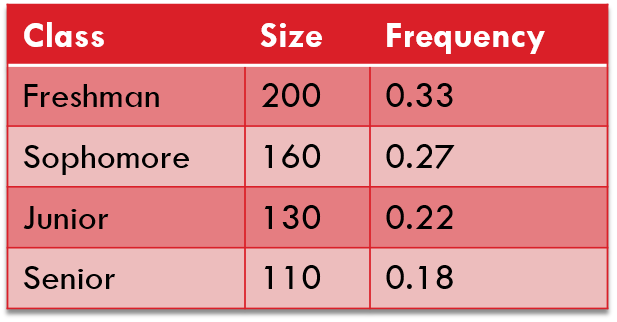
\includegraphics[width=0.8\linewidth,keepaspectratio]{mode}
%\end{center}
%\code{Calculate and verify the answer}
\end{frame}

%%%%%%%%%%%%%%%%%%%%%%%%%%%%%%%%%%%%%%%%%%%%%%%%%%%%%%%%%%
\begin{frame}[fragile]\frametitle{Mode}	
\begin{center}
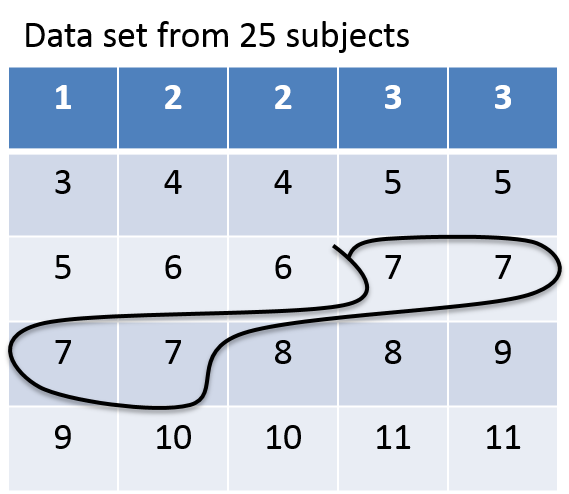
\includegraphics[width=0.6\linewidth,keepaspectratio]{da7}
\end{center}
Median = 7
\end{frame}


%%%%%%%%%%%%%%%%%%%%%%%%%%%%%%%%%%%%%%%%%%%%%%%%%%%%%%%%%%%%%%%%%%%%%%%%
\begin{frame}[fragile]\frametitle{Mode}
Implement mode
\begin{lstlisting}
def mode(datalist):
	:
	return m

lst = [9,3,7,2,7,10,23,44,12,42,19,11,22,5,3,4,3,21,3]
result = mode(lst)
print("Mode : {}".format(result))
\end{lstlisting}
Result?
\end{frame}

%%%%%%%%%%%%%%%%%%%%%%%%%%%%%%%%%%%%%%%%%%%%%%%%%%%%%%%%%%
\begin{frame}[fragile]\frametitle{Mode}
\begin{lstlisting}
def frequency_distribution(datalist):
	freqs = dict()
	for item in datalist:
		if item not in frees.keys():
			freqs[item] = 1
		else:
			freqs[item] += 1
	return freqs

def mode(datalist):
    d = frequency_distribution(datalist)
    print(d)
    most_often = 0
    m = 0
    for item in d.keys():
        if d[item] > most_often:
            most_often = d[item]
            m = item
    return m
\end{lstlisting}
Mode : 3
\end{frame}

%%%%%%%%%%%%%%%%%%%%%%%%%%%%%%%%%%%%%%%%%%%%%%%%%%%%%%%%%%
\begin{frame}[fragile]\frametitle{Mode}
Another implementation. Counter returns dictionary of frquencies and values.
\begin{lstlisting}
from collections import Counter

def mode2(x):
    counts = Counter(x)
    max_count = max(counts.values())
    return [x_i for x_i, count in counts.items() if count == max_count]  # multiple modes are possible
\end{lstlisting}
Mode : [3]
\end{frame}



%%%%%%%%%%%%%%%%%%%%%%%%%%%%%%%%%%%%%%%%%%%%%%%%%%%%%%%%%%
\begin{frame}[fragile]\frametitle{Central Tendency}	

\begin{itemize}
\item Mean: Summarizes all the information in the data set
\item Median: Splits the data sets into two halves: there are an equal number of values above and below it.
\item Mode: The most common value in the data set.
\end{itemize}

%\begin{center}
%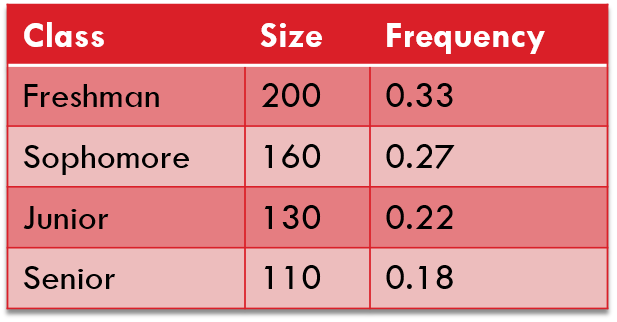
\includegraphics[width=0.8\linewidth,keepaspectratio]{mode}
%\end{center}

\end{frame}

%%%%%%%%%%%%%%%%%%%%%%%%%%%%%%%%%%%%%%%%%%%%%%%%%%%%%%%%%%
\begin{frame}[fragile]\frametitle{Locating Central Tendency}	
\begin{center}
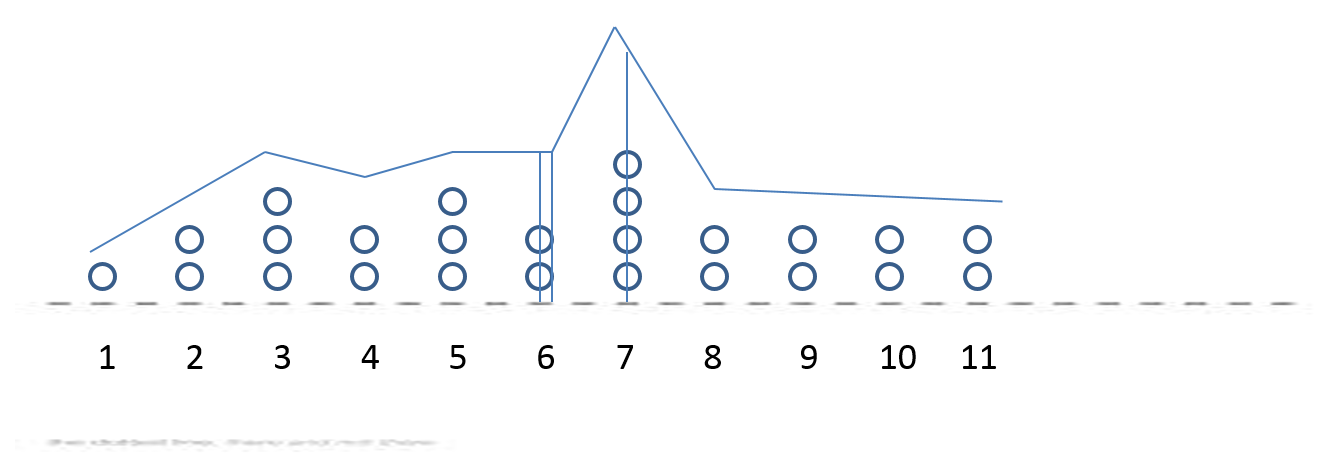
\includegraphics[width=\linewidth,keepaspectratio]{da8}
\end{center}
Mean = 6.12		

Median = 6		

Mode = 7

\end{frame}

%%%%%%%%%%%%%%%%%%%%%%%%%%%%%%%%%%%%%%%%%%%%%%%%%%%%%%%%%%%%%%%%%%%%%%%%%%%%%%%%%%
\begin{frame}[fragile]\frametitle{}
\begin{center}
{\Large Descriptive Statistics Exercise}
\end{center}
\end{frame}

%%%%%%%%%%%%%%%%%%%%%%%%%%%%%%%%%%%%%%%%%%%%%%%%%%%%%%%%%%
\begin{frame}[fragile]\frametitle{Exercise}	
Our Data
\begin{lstlisting}
lst = [9,3,7,2,7,10,23,44,12,42,19,11,22,5,3,4,3,21,3]
\end{lstlisting}

Store as list of integers and calculate Mean, Median and Mode
\end{frame}

% %%%%%%%%%%%%%%%%%%%%%%%%%%%%%%%%%%%%%%%%%%%%%%%%%%%%%%%%%%
% \begin{frame}[fragile]\frametitle{Calculate Mean}	
% % \begin{lstlisting}
% % def mean(datalist):
	% % total = 0
	% % mean = 0
	% % for item in datalist:
		% % total += item
	% % mean = total / float(len(datalist))
	% % return mean
% % \end{lstlisting}

% \code{Result?}
% \end{frame}

% %%%%%%%%%%%%%%%%%%%%%%%%%%%%%%%%%%%%%%%%%%%%%%%%%%%%%%%%%%
% \begin{frame}[fragile]\frametitle{Calculate Median}	
% % \begin{lstlisting}
% % def median(datalist):
	% % numsort = sorted(datalist)
	% % mid = len(numsort) / 2
	% % median = 1
	% % if len(numsort) % 2 == 0:
		% % median = (numsort[mid - 1] +
	% % else:
		% % median = numsort[(len(numsort) 
	% % return median
% % \end{lstlisting}

% \code{Result?}
% \end{frame}

% %%%%%%%%%%%%%%%%%%%%%%%%%%%%%%%%%%%%%%%%%%%%%%%%%%%%%%%%%%
% \begin{frame}[fragile]\frametitle{Calculate Mode}	
% % \begin{lstlisting}
% % def frequency_distribution(datalist):
	% % freqs = dict()
	% % for item in datalist:
		% % if item not in frees.keys():
			% % freqs[item] = 1
		% % else:
			% % freqs[item] += 1
	% % return freqs

% % def mode(datalist):
	% % d = frequency_distribution(datalist)
	% % most_often = 0
	% % mode = 0
	% % for item in d.keys():
		% % if d[item] > most_often:
			% % most_often = d[item]
		% % mode = item
	% % return mode
% % \end{lstlisting}

% \code{Result?}
% \end{frame}

%%%%%%%%%%%%%%%%%%%%%%%%%%%%%%%%%%%%%%%%%%%%%%%%%%%%%%%%%%%%%%%%%%%%%%%%%%%%%%%%%%
\begin{frame}[fragile]\frametitle{}
\begin{center}
{\Large Descriptive Statistics Exercise}
\end{center}
\end{frame}

%%%%%%%%%%%%%%%%%%%%%%%%%%%%%%%%%%%%%%%%%%%%%%%%%%%%%%%%%%
\begin{frame}[fragile]\frametitle{Exercise}	
\begin{lstlisting}
crater_diameter = [46, 51, 49, 82, 74, 63, 49, 70, 48, 47, 79, 48, 52, 55, 49, 51, 58, 82, 72, 45]
print mean(crater_diameter)
print median(crater_diameter)
print mode(crater_diameter)
\end{lstlisting}

\code{Result? 58.5,51.5,49}
\end{frame}


%%%%%%%%%%%%%%%%%%%%%%%%%%%%%%%%%%%%%%%%%%%%%%%%%%%%%%%%%%%%%%%%%%%%%%%%%%%%%%%%%%
\begin{frame}[fragile]\frametitle{}
\begin{center}
{\Large Measure of Spread}
\end{center}
\end{frame}

%%%%%%%%%%%%%%%%%%%%%%%%%%%%%%%%%%%%%%%%%%%%%%%%%%%%%%%%%%
\begin{frame}[fragile]\frametitle{Measure of Spread}	

\begin{itemize}
\item Range: The largest value minus the smallest value.
\item Semi-Interquartile range: One half of the difference between the 75th percentile and the 25th percentile
\item Standard Deviation:	The square root of the average of the squared deviations from the mean
\end{itemize}

%\begin{center}
%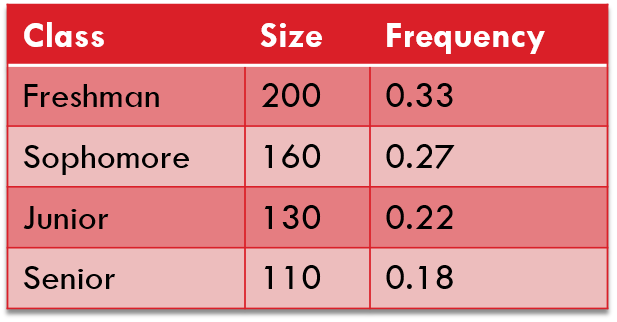
\includegraphics[width=0.8\linewidth,keepaspectratio]{mode}
%\end{center}

\end{frame}



%%%%%%%%%%%%%%%%%%%%%%%%%%%%%%%%%%%%%%%%%%%%%%%%%%%%%%%%%%
\begin{frame}[fragile]\frametitle{Range}	
\begin{itemize}
\item Variation between the smallest and the largest values
\item Can be misleading if most values are concentrated, but a few values are extreme
\end{itemize}
$range(x) = max(x) - min(x)$

\end{frame}

%%%%%%%%%%%%%%%%%%%%%%%%%%%%%%%%%%%%%%%%%%%%%%%%%%%%%%%%%%
\begin{frame}[fragile]\frametitle{Range}	
\begin{center}
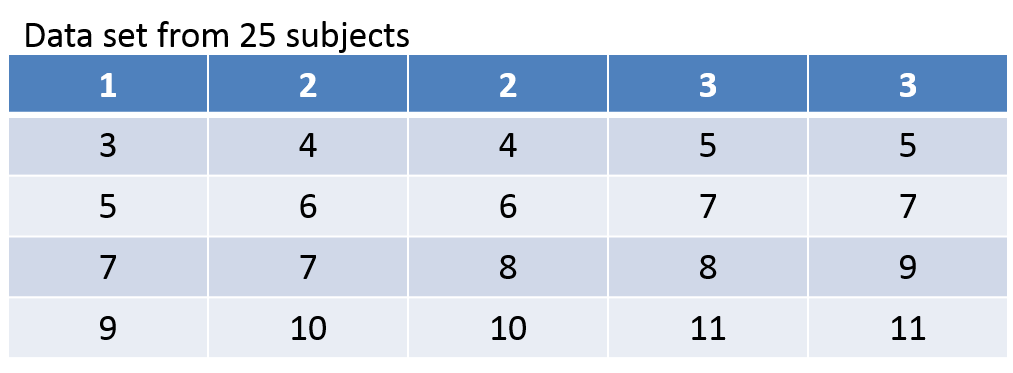
\includegraphics[width=0.6\linewidth,keepaspectratio]{da9}
\end{center}
Range = 11 -1 = 10

\begin{itemize}
\item A `quick and easy' indication of variability
\item No indication of dispersion within
\item Unstable, as depends ONLY on Outliers/Extremes
\end{itemize}
\code{Calculate and verify the answer}
\end{frame}

%%%%%%%%%%%%%%%%%%%%%%%%%%%%%%%%%%%%%%%%%%%%%%%%%%%%%%%%%%%%%%%%%%%%%%%%
\begin{frame}[fragile]\frametitle{Range}
Implement my\_range. It cannot be called as ``range'' is already there in Python, so a different name
\begin{lstlisting}
def my_range(datalist):
	:
	return min, max, diff

lst = [9,3,7,2,7,10,23,44,12,42,19,11,22,5,3,4,3,21,3]
min,max,diff = my_range(lst)
print("Range: Min {}, Max {}, Diff {}".format(min,max,diff))
\end{lstlisting}
\end{frame}

%%%%%%%%%%%%%%%%%%%%%%%%%%%%%%%%%%%%%%%%%%%%%%%%%%%%%%%%%%
\begin{frame}[fragile]\frametitle{Range}
\begin{lstlisting}
def my_range(abclist):
    smallest = abclist[0]
    largest = abclist[0]
    range_of_values = 0
    for item in abclist[1:]:
        if item < smallest:
            smallest = item
        elif item > largest:
            largest = item
    range_of_values = largest - smallest
    return smallest, largest, range_of_values
\end{lstlisting}
Range: Min 2, Max 44, Diff 42
\end{frame}

%%%%%%%%%%%%%%%%%%%%%%%%%%%%%%%%%%%%%%%%%%%%%%%%%%%%%%%%%%
\begin{frame}[fragile]\frametitle{Range}
min max functions are available on list
\begin{lstlisting}
def my_range2(x):
	return max(x) - min(x)

diff = my_range2(lst)
print("Range: {}".format(diff))	
\end{lstlisting}
Range: 42
\end{frame}



% %%%%%%%%%%%%%%%%%%%%%%%%%%%%%%%%%%%%%%%%%%%%%%%%%%%%%%%%%%
% \begin{frame}[fragile]\frametitle{Range}	
% % \begin{lstlisting}
% % def range_min_max(abclist):
    % % smallest = abclist[0]
    % % largest = abclist[0]
    % % range_of_values = 0
    % % for item in abclist[1:]:
        % % if item < smallest:
            % % smallest = item
        % % elif item > largest:
            % % largest = item
    % % range_of_values = largest - smallest
    % % return smallest, largest, range_of_values
% % \end{lstlisting}

% %\code{Result? 58.5,51.5,49}
% \end{frame}






%%%%%%%%%%%%%%%%%%%%%%%%%%%%%%%%%%%%%%%%%%%%%%%%%%%%%%%%%%
\begin{frame}[fragile]\frametitle{Percentiles}	
\begin{itemize}
\item For ordered data, percentile is useful.
\item Given an ordinal or continuous attribute x and a number p between 0 and 100, the pth percentile xp is a value of x such that p\% of the observed values are less than xp.
\item Example: the 75th percentile is the value such that 75\% of all values are less than it.
\end{itemize}

\end{frame}


%%%%%%%%%%%%%%%%%%%%%%%%%%%%%%%%%%%%%%%%%%%%%%%%%%%%%%%%%%
\begin{frame}[fragile]\frametitle{Quantile}	
Quantiles are cut points in set of data. They can represent the bottom
ten percent of the data or the top 75\% or any \% from 0 to 100.
% \begin{lstlisting}
% def quantile(datalist,num):
	% index = int(num * len(datalist)) # slicing parameter
	% if num > .5:
		% return sorted(datalist)[index:]
	% else:
		% return sorted(datalist)[:index]
% \end{lstlisting}
% quantile(lst,0.10)
% quantile(lst,0.25)
% quantile(lst,0.75)
% quantile(lst,0.90)
% \code{Result?[2],[2,3,3,3],[21,22,23,42,44],[42,44] }
\end{frame}


%%%%%%%%%%%%%%%%%%%%%%%%%%%%%%%%%%%%%%%%%%%%%%%%%%%%%%%%%%%%%%%%%%%%%%%%
\begin{frame}[fragile]\frametitle{Quantile}
Implement quantile
\begin{lstlisting}
def quantile(datalist):
	:
	return q

def interquartile_range(x):
	:
	return iqr
	
lst = [9,3,7,2,7,10,23,44,12,42,19,11,22,5,3,4,3,21,3]
result1 = quantile(lst,0.10)
result2 = quantile(lst,0.25)
result3 = quantile(lst,0.75)
result4 = quantile(lst,0.90)
result5 = interquartile_range(lst)
print("Q10 {}, Q25 {}, Q50 {} Q90 {} IQR {}".format(result1,result2,result3,result4,result5))
\end{lstlisting}
\end{frame}


%%%%%%%%%%%%%%%%%%%%%%%%%%%%%%%%%%%%%%%%%%%%%%%%%%%%%%%%%%
\begin{frame}[fragile]\frametitle{Quantile}
\begin{lstlisting}
def quantile(datalist,num):
    index = int(num * len(datalist)) # slicing parameter
    return sorted(datalist)[index]
    # For values :
    # if num > .5:
    #     return sorted(datalist)[index:]
    # else:
    #     return sorted(datalist)[:index]

def interquartile_range(x):
    return	quantile(x, 0.75) - quantile(x, 0.25)
\end{lstlisting}
\# Q10 [2], Q25 [2, 3, 3, 3], Q50 [21, 22, 23, 42, 44] Q90 [42, 44]
Q10 3, Q25 3, Q50 21 Q90 42 IQR 18
\end{frame}

%%%%%%%%%%%%%%%%%%%%%%%%%%%%%%%%%%%%%%%%%%%%%%%%%%%%%%%%%%
\begin{frame}[fragile]\frametitle{Semi-Interquartile Range}	
\begin{itemize}
\item Quartiles are Quantiles at 25\% and 75\%.
\item Inter Quartile Range (IQR) is between 25\% and 75\%.
\item More resistant to extreme values than the range
\item Does not utilize all the values in the data or set for its computation
\item If small, the values are concentrated near the median
\end{itemize}
\end{frame}

%%%%%%%%%%%%%%%%%%%%%%%%%%%%%%%%%%%%%%%%%%%%%%%%%%%%%%%%%%
\begin{frame}[fragile]\frametitle{Semi-Interquartile Range}	
\begin{itemize}
\item 75th percentile: the value in the date set which is exceeded by 75\% of the total number of items in the set
\item 25 x (0.75) = 18.75
\item 18.75 : rank of the 75th percentile
\item 18th  and 19th items, both  8
\item 75th percentile = 8
\end{itemize}
\begin{center}
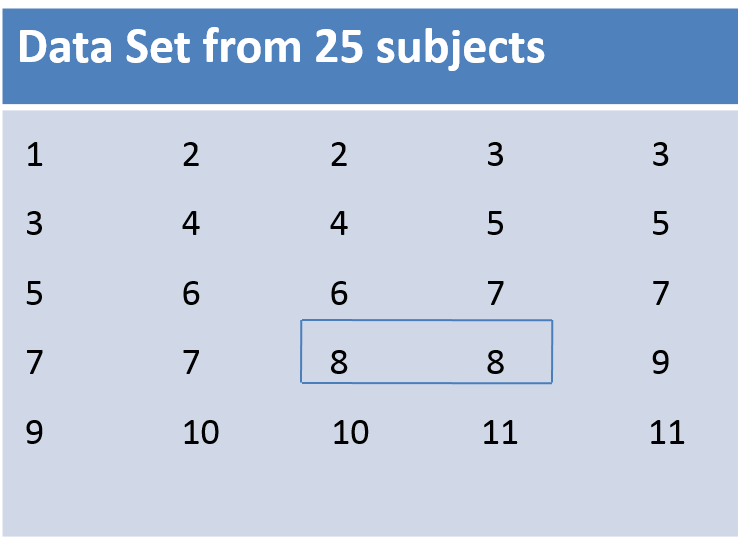
\includegraphics[width=0.4\linewidth,keepaspectratio]{da13}
\end{center}
\end{frame}


%%%%%%%%%%%%%%%%%%%%%%%%%%%%%%%%%%%%%%%%%%%%%%%%%%%%%%%%%%
\begin{frame}[fragile]\frametitle{Semi-Interquartile Range}	
\begin{itemize}
\item 25th percentile: the value in the date set which is exceeded by 75\% of the total number of items in the set
\item 25 x (0.25) = 6.25
\item 6.25 : rank of the 25th percentile
\item 6th item = 3 and 7th item = 4
\item 25th percentile = 3 + (0.25)(4-3)
\item 25th percentile = 3.25
\end{itemize}
\begin{center}
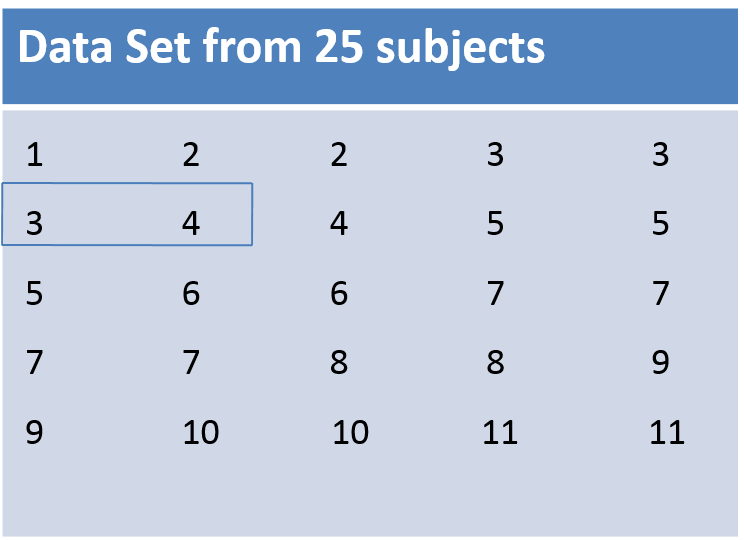
\includegraphics[width=0.4\linewidth,keepaspectratio]{da14}
\end{center}
\code{Calculate and verify the answer}
\end{frame}


%%%%%%%%%%%%%%%%%%%%%%%%%%%%%%%%%%%%%%%%%%%%%%%%%%%%%%%%%%
\begin{frame}[fragile]\frametitle{Semi-Interquartile Range}	
\begin{itemize}
\item 75th percentile = 8
\item 25th percentile = 3.25
\item SIQR =1/2 (8 - 3.25)
\item SIQR = 2.375
\item Semi-interquartile range = 2.375
\end{itemize}

\begin{center}
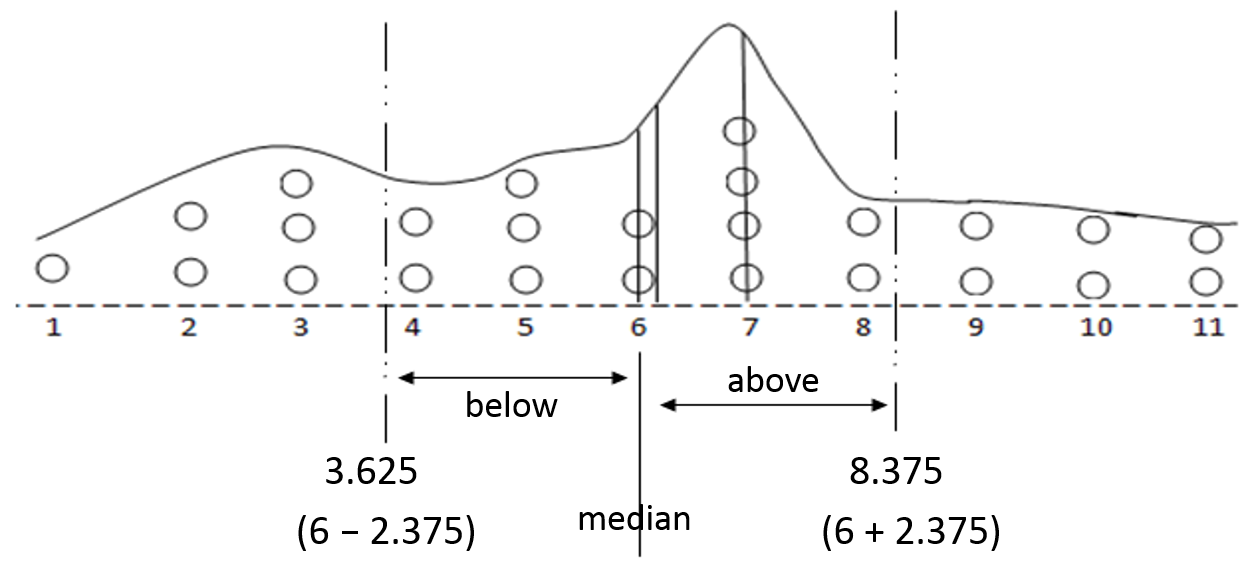
\includegraphics[width=0.8\linewidth,keepaspectratio]{da10}
\end{center}
%\code{Calculate and verify the answer}
\end{frame}



%%%%%%%%%%%%%%%%%%%%%%%%%%%%%%%%%%%%%%%%%%%%%%%%%%%%%%%%%%
\begin{frame}[fragile]\frametitle{Standard Deviation}	
\begin{itemize}
\item How far each value if from the mean
\item Uses all the values in the data for its computation
\item If small, the values are concentrated near the mean.
\item If LARGE, the values are scattered widely about the mean
\item z score: how many std deviations from the mean.
\end{itemize}
\begin{center}
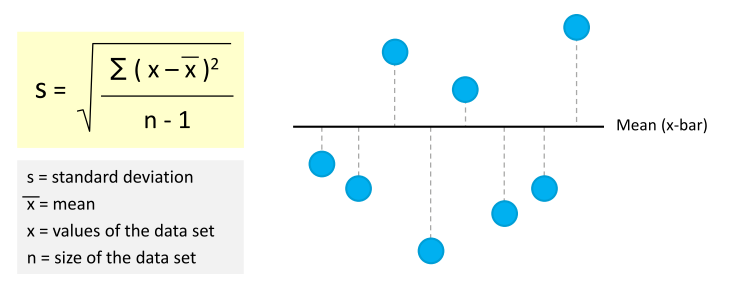
\includegraphics[width=\linewidth,keepaspectratio]{da16}
\end{center}
\end{frame}


%%%%%%%%%%%%%%%%%%%%%%%%%%%%%%%%%%%%%%%%%%%%%%%%%%%%%%%%%%%%%%%%%%%%%%%%
\begin{frame}[fragile]\frametitle{Variance, Standard Deviation}
Implement variance and standard deviation.
\begin{center}
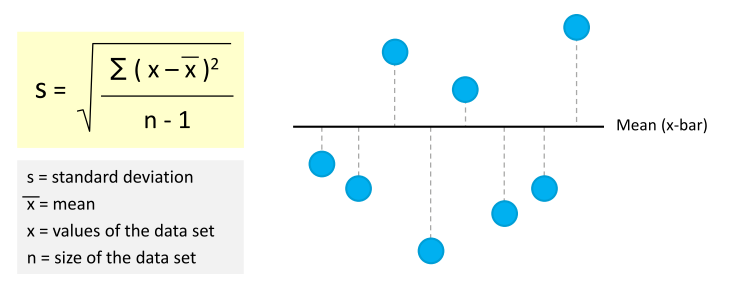
\includegraphics[width=0.5\linewidth,keepaspectratio]{da16}
\end{center}

\begin{lstlisting}
def variance(datalist):
	:
	return v

def std_dev(datalist):
	:
	return s

lst = [9,3,7,2,7,10,23,44,12,42,19,11,22,5,3,4,3,21,3]
result1 = variance(lst)
result2 = std_dev(lst)
print("Variance {}, Std Dev {}".format(result1,result2))
\end{lstlisting}
\end{frame}


% %%%%%%%%%%%%%%%%%%%%%%%%%%%%%%%%%%%%%%%%%%%%%%%%%%%%%%%%%%
% \begin{frame}[fragile]\frametitle{Calculate Deviation}	
% \begin{lstlisting}
% def mean(datalist):
    % total = 0
    % mean = 0
    % for item in datalist:
        % total += item
    % mean = total / float(len(datalist))
    % return mean
 
% def avg_dev(thislist):
    % average = mean(thislist)
    % sum_of_dev = 0
    % avg_dev = 0
    % for item in thislist:
        % sum_of_dev += abs((average - item))
    % avg_dev = sum_of_dev / len(thislist)
    % return avg_dev
% \end{lstlisting}
% \end{frame}


%%%%%%%%%%%%%%%%%%%%%%%%%%%%%%%%%%%%%%%%%%%%%%%%%%%%%%%%%%
\begin{frame}[fragile]\frametitle{Standard Deviation}	
To reparametrize Covariance value between -1 and 1, need to divide by std devs. Empirical Rule for symmetric bell-shaped distributions
\begin{itemize}
\item About 68\% of the values will lie within 1 standard deviation of the mean
\item About 95\% of the values will lie Within 2 standard deviation 
\item About 99.7\% of the values will lie within 3 standard deviation of the mean
\end{itemize}
$variance(x) = s_x^2 = 1/(n-1)\sum (x_i - \bar{x})^2$
$sd(x) = s_x = \sqrt{1/(n-1)\sum (x_i - \bar{x})^2}$
\end{frame}

% %%%%%%%%%%%%%%%%%%%%%%%%%%%%%%%%%%%%%%%%%%%%%%%%%%%%%%%%%%
% \begin{frame}[fragile]\frametitle{Calculate Deviation}	
% \begin{lstlisting}
% def variance(thatlist):
    % average = mean(thatlist)
    % sum_of_sqrt_dev = 0
    % variance = 0
    % for item in thatlist:
        % sum_of_sqrt_dev += (average - item) ** 2
    % variance = sum_of_sqrt_dev / len(thatlist)
    % return variance
 
% def std_dev(anotherlist):
    % std_dev = variance(anotherlist) ** 0.5
    % return std_dev
% \end{lstlisting}
% \end{frame}


%%%%%%%%%%%%%%%%%%%%%%%%%%%%%%%%%%%%%%%%%%%%%%%%%%%%%%%%%%
\begin{frame}[fragile]\frametitle{Variance, Standard Deviation}
\begin{lstlisting}
def de_mean(x):
	"""translate x by subtracting its mean"""
	x_bar = mean(x)
	return	[x_i - x_bar for x_i in x]

def sum_of_squares(diffs):
	sum_of_squares = 0
	for df in diffs:
          sum_of_squares += (df) ** 2
     return sum_of_squares

def variance(x):
	"""assumes x has at	least two elements"""
	n = len(x)
	deviations = de_mean(x)
	return	sum_of_squares(deviations) / (n - 1)
 
def std_dev(anotherlist):
	std_dev = variance(anotherlist) ** 0.5
	return std_dev
\end{lstlisting}
Variance 158.36257309941527, Std Dev 12.584219208970229
\end{frame}


%%%%%%%%%%%%%%%%%%%%%%%%%%%%%%%%%%%%%%%%%%%%%%%%%%%%%%%%%%%
%\begin{frame}[fragile]\frametitle{Standard Deviation}	
%Mean = 6.12
%Standard Deviation = 2.934
%\begin{center}
%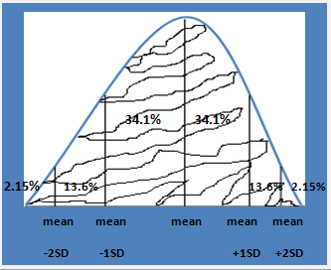
\includegraphics[width=0.6\linewidth,keepaspectratio]{da11}
%\end{center}
%\code{Calculate and verify the answer}
%\end{frame}

%%%%%%%%%%%%%%%%%%%%%%%%%%%%%%%%%%%%%%%%%%%%%%%%%%%%%%%%%%
\begin{frame}[fragile]\frametitle{Standard Deviation}	
Standard Deviation = 2.934
\begin{center}
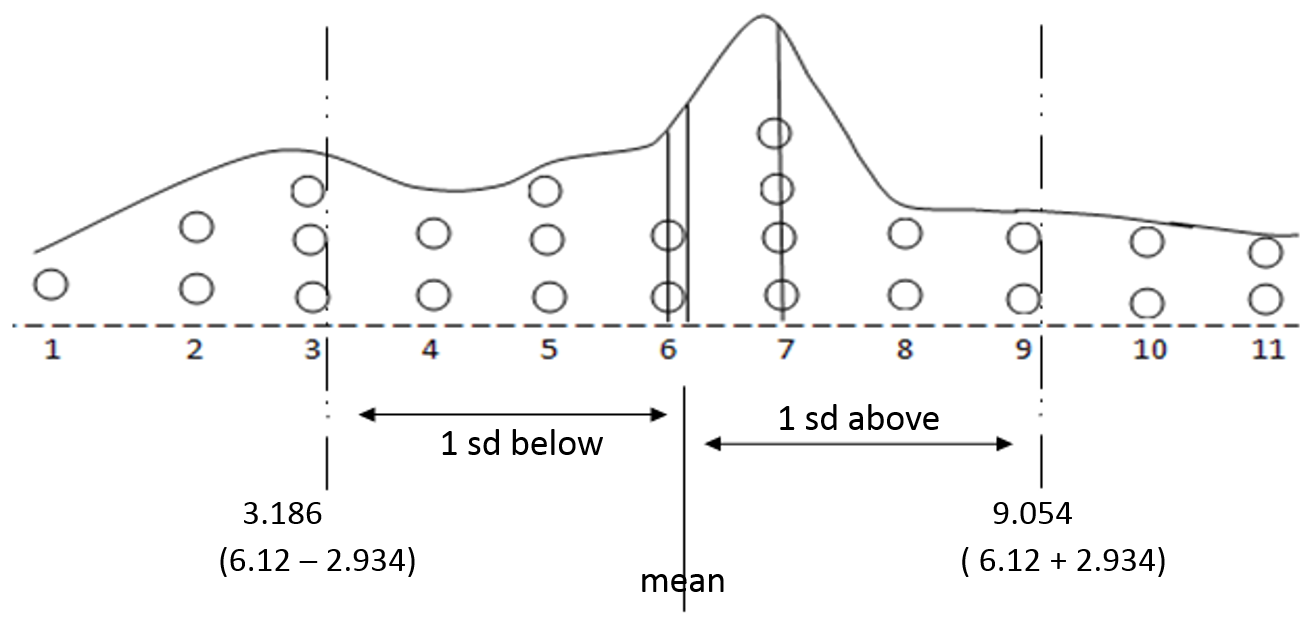
\includegraphics[width=\linewidth,keepaspectratio]{da12}
\end{center}
\end{frame}

%%%%%%%%%%%%%%%%%%%%%%%%%%%%%%%%%%%%%%%%%%%%%%%%%%%%%%%%%%%%%%%%%%%%%%%%%%%%%%%%%%
\begin{frame}[fragile]\frametitle{}
\begin{center}
{\Large Descriptive Statistics Exercise}
\end{center}
\end{frame}

%%%%%%%%%%%%%%%%%%%%%%%%%%%%%%%%%%%%%%%%%%%%%%%%%%%%%%%%%%
\begin{frame}[fragile]\frametitle{Exercise}	
\begin{lstlisting}
crater_diameter = [46, 51, 49, 82, 74, 63, 49, 70, 48, 47, 79, 48, 52, 55, 49, 51, 58, 82, 72, 45]
 
print range_min_max(crater_diameter)
print avg_dev(crater_diameter)
print variance(crater_diameter)
print std_dev(crater_diameter)
\end{lstlisting}
\code{Result?(45,82,37),11.25,161.45,12.7062 }
\end{frame}


%%%%%%%%%%%%%%%%%%%%%%%%%%%%%%%%%%%%%%%%%%%%%%%%%%%%%%%%%%
\begin{frame}[fragile]\frametitle{Exercise}	
Find the mean, median, range and standard deviation for the following set of data:

\lstinline|2.8, 8.7, 0.7, 4.9, 3.4, 2.1 & 4.0|
\end{frame}

%%%%%%%%%%%%%%%%%%%%%%%%%%%%%%%%%%%%%%%%%%%%%%%%%%%%%%%%%%
\begin{frame}[fragile]\frametitle{Exercise}	
Find the mean, median, range and standard deviation for the following set of data:

\begin{center}
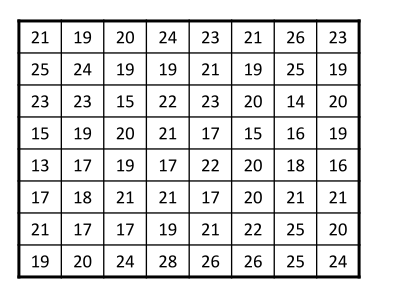
\includegraphics[width=0.6\linewidth,keepaspectratio]{da17}
\end{center}
\end{frame}

%
%%%%%%%%%%%%%%%%%%%%%%%%%%%%%%%%%%%%%%%%%%%%%%%%%%%%%%%%%%%%%%%%%%%%%%%%
\begin{frame}[fragile]\frametitle{Difference between Standard Deviation and Standard Error}
\begin{columns}
    \begin{column}[T]{0.6\linewidth}
	\begin{itemize}
	\item For a set of normally distributed observations you have mean and standard deviation.
	\item If you do this for different samples, you get their own respective means and standard deviations.
	\end{itemize}

    \end{column}
    \begin{column}[T]{0.4\linewidth}
      \begin{center}
      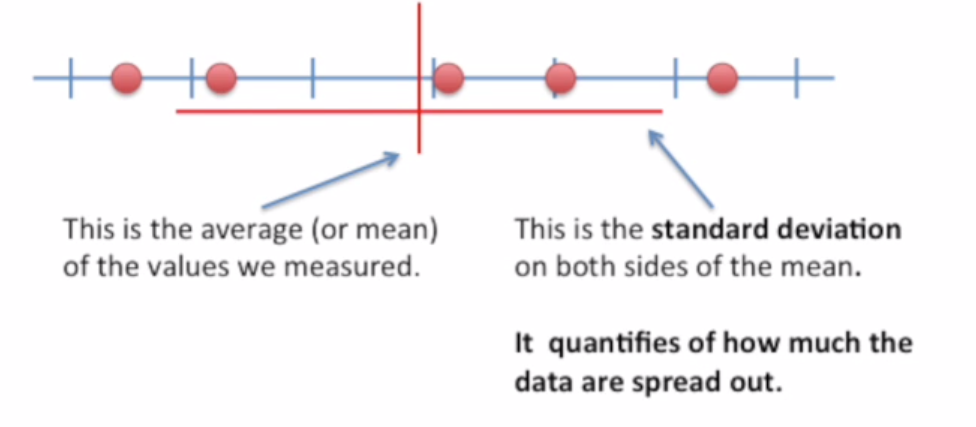
\includegraphics[width=\linewidth,keepaspectratio]{statq28}
	  
	  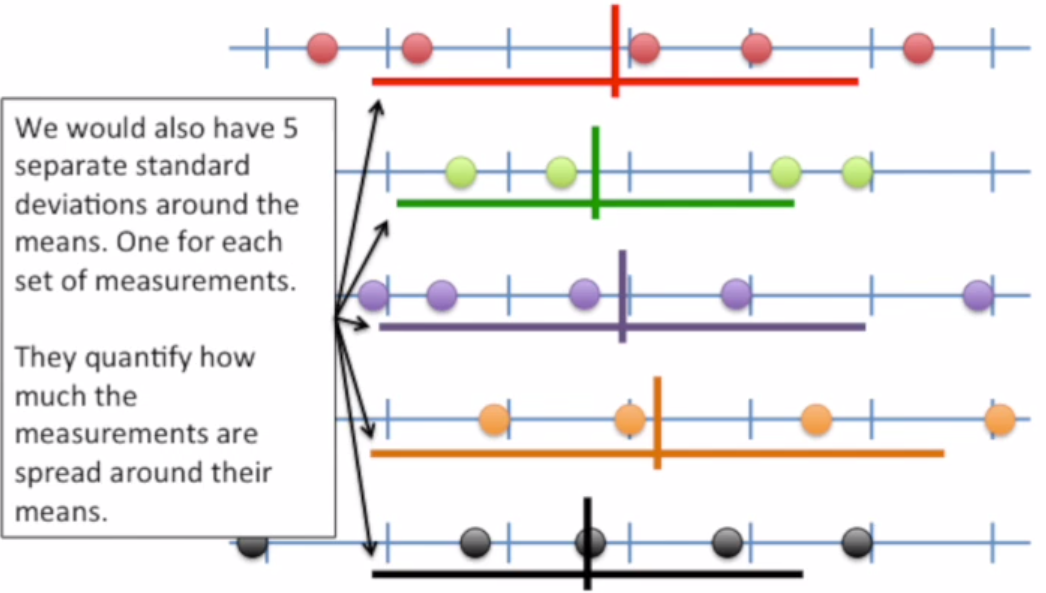
\includegraphics[width=\linewidth,keepaspectratio]{statq29}
	   
	  	\end{center}
    \end{column}

  \end{columns}
  
\tiny{(Ref: StatQuest: Difference between Standard Deviation and Standard Error - Josh Starmer )}
\end{frame}

%%%%%%%%%%%%%%%%%%%%%%%%%%%%%%%%%%%%%%%%%%%%%%%%%%%%%%%%%%%%%%%%%%%%%%%%
\begin{frame}[fragile]\frametitle{Difference between Standard Deviation and Standard Error}

	\begin{itemize}
	\item Plotting those sample means, and sample standard deviations, can form another (meta?) distribution
	\item Standard deviation of this meta distribution is called Standard Error
	\end{itemize}

      \begin{center}
      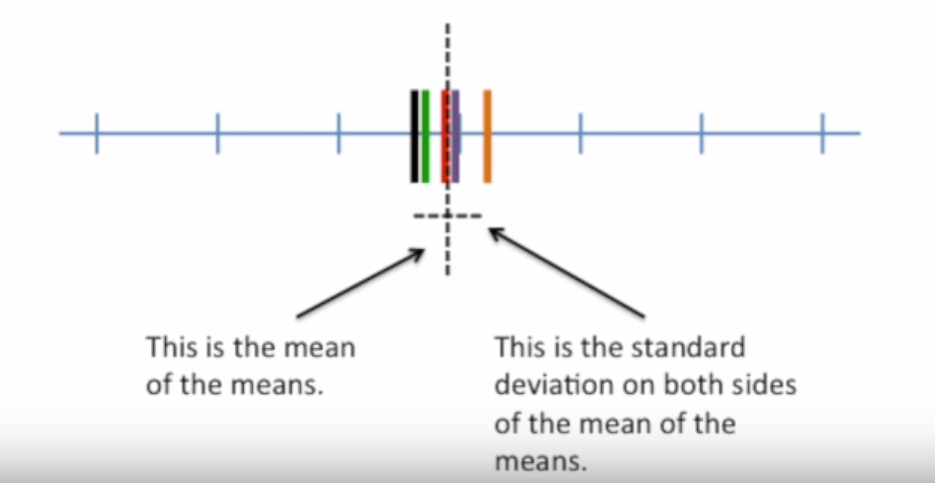
\includegraphics[width=0.8\linewidth,keepaspectratio]{statq30}
	\end{center}

  
\tiny{(Ref: StatQuest: Difference between Standard Deviation and Standard Error - Josh Starmer )}
\end{frame}

%%%%%%%%%%%%%%%%%%%%%%%%%%%%%%%%%%%%%%%%%%%%%%%%%%%%%%%%%%%%%%%%%%%%%%%%%%%%%%%%%%
\begin{frame}[fragile]\frametitle{}
\begin{center}
{\Large Measure of Asymmetry}
\end{center}
\end{frame}

%%%%%%%%%%%%%%%%%%%%%%%%%%%%%%%%%%%%%%%%%%%%%%%%%%%%%%%%%%
\begin{frame}[fragile]\frametitle{Measures of Shape}	
\begin{itemize}
\item  To have a general idea of its shape, or distribution
\item Helps identifying which descriptive statistic to use
\item  Symmetrical or nonsymmetrical
\item Skewness.
\item Kurtosis.
\end{itemize}
\begin{center}
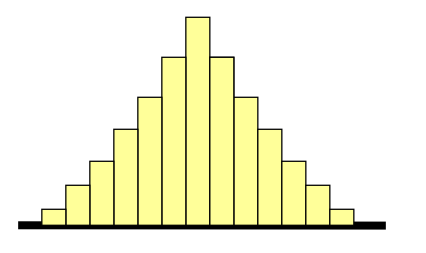
\includegraphics[width=0.6\linewidth,keepaspectratio]{da18}
\end{center}
\end{frame}

%%%%%%%%%%%%%%%%%%%%%%%%%%%%%%%%%%%%%%%%%%%%%%%%%%%%%%%%%%
\begin{frame}[fragile]\frametitle{Symmetric}	
\begin{itemize}

\item  Uniform.
\item  Normal.
\item  Camel-back.
\item  Bow-tie shaped.
\end{itemize}
\begin{center}
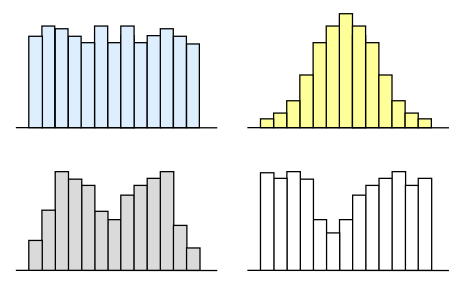
\includegraphics[width=0.6\linewidth,keepaspectratio]{da19}
\end{center}
\end{frame}

%%%%%%%%%%%%%%%%%%%%%%%%%%%%%%%%%%%%%%%%%%%%%%%%%%%%%%%%%%
\begin{frame}[fragile]\frametitle{Skewness}	
Measures the degree to which the values are symmetrically distributed about the center
\begin{center}
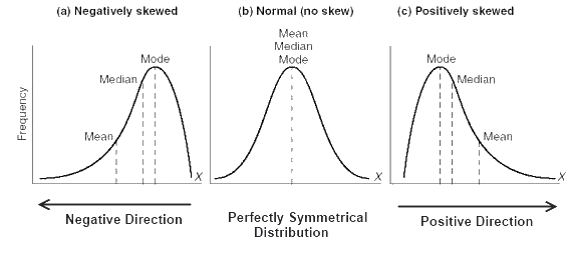
\includegraphics[width=0.8\linewidth,keepaspectratio]{skewness}
\end{center}
If the distribution of values is skewed, then the median is a better indicator of the middle, compare to the mean.
\end{frame}

%%%%%%%%%%%%%%%%%%%%%%%%%%%%%%%%%%%%%%%%%%%%%%%%%%%%%%%%%%
\begin{frame}[fragile]\frametitle{Skewness}	
For perfectly symmetrical distribution, like Normal Distribution (middle figure):
\begin{center}
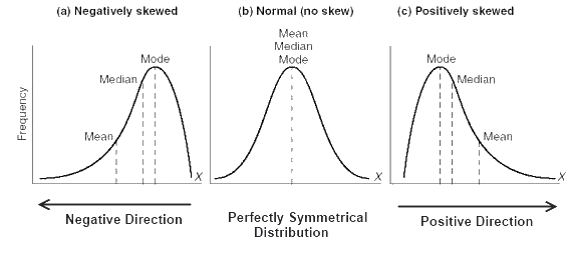
\includegraphics[width=0.8\linewidth,keepaspectratio]{skewness}
\end{center}
\begin{itemize}
\item  Whats the mean?: the middle axis point
\item Whats the mode?: Highest frequency, top most point
\item Whats the median?: Half split of the curve is at the middle.
\end{itemize}
All Points/Axes are same.
\end{frame}

%%%%%%%%%%%%%%%%%%%%%%%%%%%%%%%%%%%%%%%%%%%%%%%%%%%%%%%%%%
\begin{frame}[fragile]\frametitle{Skewness}	
For skewed distribution (left and right figures):
\begin{center}
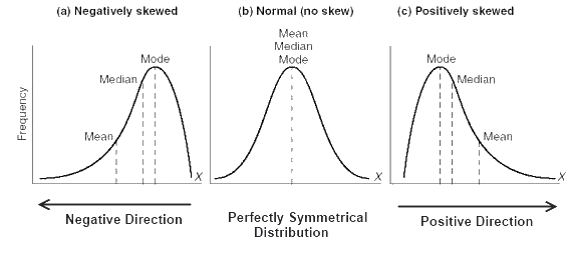
\includegraphics[width=0.8\linewidth,keepaspectratio]{skewness}
\end{center}
\begin{itemize}
\item Whats the mean?: towards tail, as most of the heavy (+ve or -ve) points are there
\item Whats the mode?: Highest frequency, top most point
\item Whats the median?: somewhere between these two
\end{itemize}
All Points/Axes are different. Sides of Mean and Mode can decide right/left skewness.
\end{frame}

%%%%%%%%%%%%%%%%%%%%%%%%%%%%%%%%%%%%%%%%%%%%%%%%%%%%%%%%%%
\begin{frame}[fragile]\frametitle{Pearson's Skewness Coefficient}	
Karl Pearson coefficient of Skewness 
$sk_p = \frac{3(\mu - median)}{\sigma}$

\begin{itemize}
\item  The direction of skewness is given by the sign.
\item The coefficient compares the sample distribution with a normal distribution. The larger the value, the larger the difference.
\item A value of zero means no skewness at all.
\item A large negative value means the distribution is negatively skewed.
\item A large positive value means the distribution is positively skewed.
\end{itemize}

\end{frame}

%%%%%%%%%%%%%%%%%%%%%%%%%%%%%%%%%%%%%%%%%%%%%%%%%%%%%%%%%%
\begin{frame}[fragile]\frametitle{3rd Moment Skewness Coefficient}	
$sk_t = \frac{\sum (x_i - \mu)^3}{\sigma^3}$

\begin{itemize}
\item If the power would have been 1 (instead of 3) then $\sum (x_i -\mu)$ would have been 0. +ve and -ve will cancel each other.
\item  Odd moments are increased when there is a long tail to the right and decreased when there is a long tail to the left. 
\end{itemize}

\end{frame}

%%%%%%%%%%%%%%%%%%%%%%%%%%%%%%%%%%%%%%%%%%%%%%%%%%%%%%%%%%
\begin{frame}[fragile]\frametitle{Skewness}	
\begin{itemize}
\item  Zero indicates perfect symmetry
\item  Negative value implies left-skewed data
\item Positive value implies right-skewed data.
\end{itemize}
\begin{center}
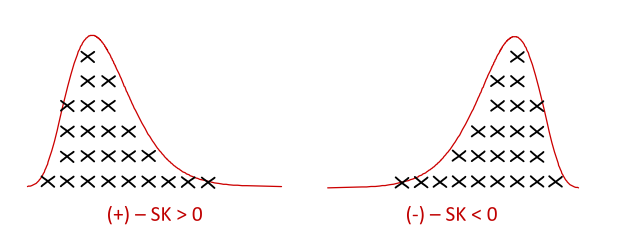
\includegraphics[width=\linewidth,keepaspectratio]{da20}
\end{center}
\end{frame}

%%%%%%%%%%%%%%%%%%%%%%%%%%%%%%%%%%%%%%%%%%%%%%%%%%%%%%%%%%%%%%%%%%%%%%%%%%%%%%%%%%
\begin{frame}[fragile]\frametitle{}
\begin{center}
{\Large Measure of Skewness}
\end{center}
\end{frame}


%%%%%%%%%%%%%%%%%%%%%%%%%%%%%%%%%%%%%%%%%%%%%%%%%%%%%%%%%%
\begin{frame}[fragile]\frametitle{Kurtosis}	
\begin{itemize}
\item  Measures the degree of flatness (or peakness)
\item Clustered around middle? More peak, more kurtosis value
\item If values spread evenly, flatted, less kurtosis value
\end{itemize}
\begin{center}
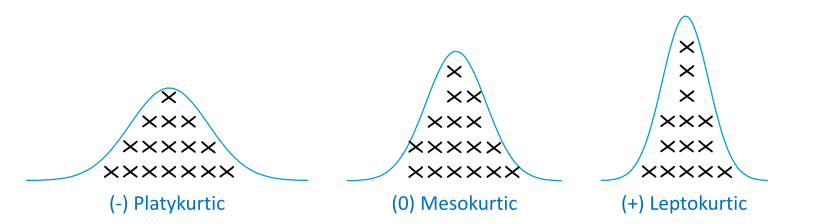
\includegraphics[width=\linewidth,keepaspectratio]{da21}
\end{center}
\end{frame}

%%%%%%%%%%%%%%%%%%%%%%%%%%%%%%%%%%%%%%%%%%%%%%%%%%%%%%%%%%
\begin{frame}[fragile]\frametitle{Kurtosis Skewness Coefficient}	
$sk_k = \frac{\sum (x_i - \mu)^4}{\sigma^4}$

\begin{itemize}
\item Since the exponent in the above is 4, the term in the summation will always be positive 
\item Moments of even order are increased when either tail is long. 
\item Kurtosis is a measure of outlier content. High if longer the tails so more the outliers.
\item The third and fourth moments are the smallest examples of these so are used for skewness and kurtosis measures.
\end{itemize}
\end{frame}

% %%%%%%%%%%%%%%%%%%%%%%%%%%%%%%%%%%%%%%%%%%%%%%%%%%%%%%%%%%
% \begin{frame}[fragile]\frametitle{Weighted Average}	
% \begin{center}
% 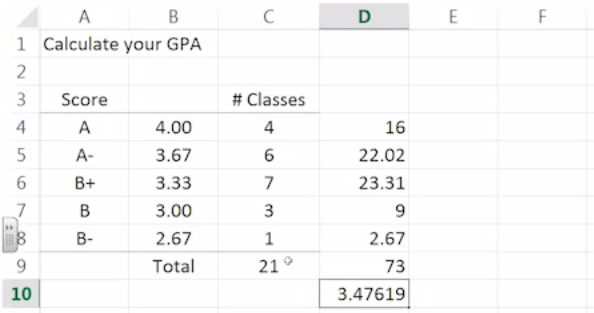
\includegraphics[width=0.7\linewidth,keepaspectratio]{wtavrg}
% \end{center}
% \end{frame}
%%%%%%%%%%%%%%%%%%%%%%%%%%%%%%%%%%%%%%%%%%%%%%%%%%%%%%%%%%%%%%%%%%%%%%%%%%%%%%%%%%
\begin{frame}[fragile]\frametitle{}
\begin{center}
{\Large Bi-variate Analysis}
\end{center}
\end{frame}

%%%%%%%%%%%%%%%%%%%%%%%%%%%%%%%%%%%%%%%%%%%%%%%%%%%%%%%%%%
\begin{frame}[fragile]\frametitle{Bi-variate Analysis}	
\begin{center}
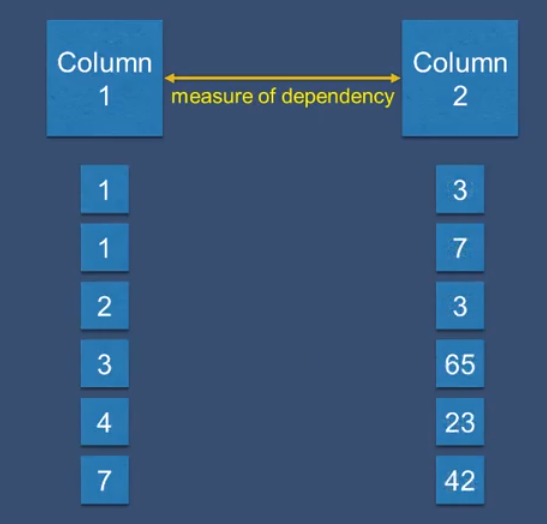
\includegraphics[width=0.7\linewidth,keepaspectratio]{bivar}
\end{center}
\end{frame}

%%%%%%%%%%%%%%%%%%%%%%%%%%%%%%%%%%%%%%%%%%%%%%%%%%%%%%%%%%%%%%%%%%%%%%%%%%%%%%%%%%
\begin{frame}[fragile]\frametitle{}

\begin{center}
{\large Correlations and Covariance}
\end{center}
\end{frame}


%%%%%%%%%%%%%%%%%%%%%%%%%%%%%%%%%%%%%%%%%%%%%%%%%%%%%%%%%%%
\begin{frame}[fragile]\frametitle{Covariance and Correlation}
Both show association between two variables
\begin{itemize}
\item Positive: If one goes up, the other does too and vice versa.
\item Example: Height and weight
\item Not always, but tendency
\item Another example: Temperature and Ice-creame sales
\item Negative: Temperature and sale of woolen clothes
\end{itemize}
\end{frame}

%%%%%%%%%%%%%%%%%%%%%%%%%%%%%%%%%%%%%%%%%%%%%%%%%%%%%%%%%%%
\begin{frame}[fragile]\frametitle{Correlation}
\begin{itemize}
\item Correlation is a value standardized between -1 to 1
\item Relation between two variables is linear, 
\item Directly proportional in case of Positive Corr
\item Inversely proportional in case of Negative Corr
\item The value of corr is the factor of proportionality
\item No correlation, ie no dependence so value = 0
\end{itemize}
\end{frame}

%%%%%%%%%%%%%%%%%%%%%%%%%%%%%%%%%%%%%%%%%%%%%%%%%%%%%%%%%%%
\begin{frame}[fragile]\frametitle{Covariance and Correlation}
\begin{center}
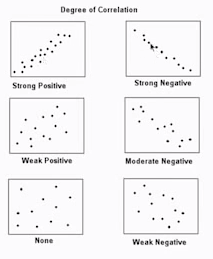
\includegraphics[width=0.55\linewidth,keepaspectratio]{corrplot}
\end{center}
\end{frame}

%%%%%%%%%%%%%%%%%%%%%%%%%%%%%%%%%%%%%%%%%%%%%%%%%%%%%%%%%%%%%%%%%%%%%%%%
\begin{frame}[fragile]\frametitle{Covariance}
Implement covariance, the paired analogue of variance.
The variance measures how a single variable deviates from its mean, covariance measures how two variables vary in tandem from their means.
\begin{center}
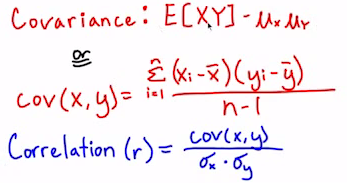
\includegraphics[width=0.5\linewidth,keepaspectratio]{corrcov}
\end{center}
\begin{lstlisting}
x = [2, 3, 0, 1, 3]
y = [ 2, 1, 0, 1, 2]
result1 = covariance(x,y)
result2 = correlation(x,y)print("CoVariance {}, Correlation {}".format(result1,result2))
\end{lstlisting}
\end{frame}

%%%%%%%%%%%%%%%%%%%%%%%%%%%%%%%%%%%%%%%%%%%%%%%%%%%%%%%%%%
\begin{frame}[fragile]\frametitle{Covariance}
Covariance is like a dot product and tell how two quantities (centered, meaning subtracted by Mean) are together/similar.
\begin{lstlisting}
def elemwise_multi(v, w):
    """v_1 * w_1 + ... + v_n * w_n"""
    return sum(v_i * w_i for v_i, w_i in zip(v, w))

def covariance(x, y):
	n = len(x)
	return	elemwise_multi(de_mean(x), de_mean(y)) / (n - 1)

\end{lstlisting}
CoVariance 0.8
\end{frame}

%%%%%%%%%%%%%%%%%%%%%%%%%%%%%%%%%%%%%%%%%%%%%%%%%%%%%%%%%%
\begin{frame}[fragile]\frametitle{Correlation}
Covariance is like a dot product normalized by standard deviation.
\begin{lstlisting}
def correlation(x, y):
	stdev_x = std_dev(x)
  	stdev_y = std_dev(y)
	if stdev_x > 0 and stdev_y > 0:
		return	covariance(x, y) / stdev_x / stdev_y
	else:
		return	0 # if	no variation, correlation is zero
\end{lstlisting}
Correlation 0.7333587976225691
\end{frame}

%%%%%%%%%%%%%%%%%%%%%%%%%%%%%%%%%%%%%%%%%%%%%%%%%%%%%%%%%%%%%%%%%%%%%%%%
\begin{frame}[fragile]\frametitle{$R^2$}

	\begin{itemize}
	\item Correlation, the regular `R' has values from -1 to 1 and is good enough to tell you that the two quantitative variables are strongly related.
	\item Why do you need $R^2$ then?
	\item Plain $R$ is not easier to interpret. 
	\item Example: $R=0.7$ is twice as good as $R=0.5$
	\item But its more clear when $R^2 = 0.7$ is 1.4 times as good as $R^2=.5$
	\end{itemize}
  
\tiny{(Ref: StatQuest: R-squared explained - Josh Starmer )}
\end{frame}

%%%%%%%%%%%%%%%%%%%%%%%%%%%%%%%%%%%%%%%%%%%%%%%%%%%%%%%%%%%%%%%%%%%%%%%%
\begin{frame}[fragile]\frametitle{$R^2$}

\begin{columns}
    \begin{column}[T]{0.6\linewidth}
	\begin{itemize}
	\item $R^2$ is used to decide the quality of the linear fitting.
	\item $Var(mean)$ represents the variation of just the mean line, ie black line.
	\item $Var(line)$ represents the variation calculated using he fitted line, ie blue line.
	\item Taking just relative ratio to make $R^2$ in range 0 t 1 and as a percentage.
	\item If the value is 0.81, it means there is 81\% less variation around fitted line than the benchmark black line.
	\item So, if one variable is input (size) and one is output (weight), then we say that 81\% of weight variation is explained by size.
	\end{itemize}

    \end{column}
    \begin{column}[T]{0.4\linewidth}
      \begin{center}
      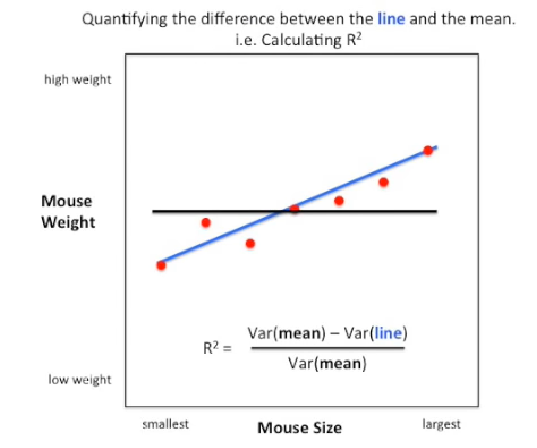
\includegraphics[width=\linewidth,keepaspectratio]{statq31}
	  
	   
	  	\end{center}
    \end{column}

  \end{columns}
  
	
\tiny{(Ref: StatQuest: R-squared explained - Josh Starmer )}
\end{frame}



%%%%%%%%%%%%%%%%%%%%%%%%%%%%%%%%%%%%%%%%%%%%%%%%%%%%%%%%%%%%%%%%%%%%%%%%%%%%%%%%%%
\begin{frame}[fragile]\frametitle{}
\begin{center}
{\Large Distributions}
\end{center}
\end{frame}


%%%%%%%%%%%%%%%%%%%%%%%%%%%%%%%%%%%%%%%%%%%%%%%%%%%%%%%%%%%%%%%%%%%%%%%%
\begin{frame}[fragile]\frametitle{What is a Statistical Distribution?}

Example
\begin{columns}
    \begin{column}[T]{0.6\linewidth}
	\begin{itemize}
	\item Say, we are measuring height of people and we plotted histogram.
	\item Measurements in the middle are more than at the ends (extreme values).
	\item If we decrease the bin size to very small width, and with lots of observations, we will get a continuous curve approximating the tops.
	\item The curve gives a general sense, so we still can calculate frequencies of the missing observations.
	\end{itemize}

    \end{column}
    \begin{column}[T]{0.4\linewidth}
      \begin{center}
      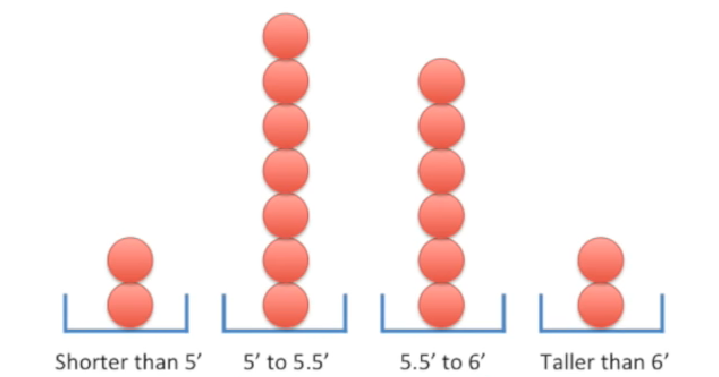
\includegraphics[width=\linewidth,keepaspectratio]{statq10}
	  
	  \includegraphics[width=\linewidth,keepaspectratio]{statq11}
	  
	  \includegraphics[width=\linewidth,keepaspectratio]{statq12}	  
	  	\end{center}
    \end{column}

  \end{columns}
  
Thats `normal' distribution.

\tiny{(Ref: StatQuest: What is a statistical distribution? - Josh Starmer )}
\end{frame}


%%%%%%%%%%%%%%%%%%%%%%%%%%%%%%%%%%%%%%%%%%%%%%%%%%%%%%%%%%%%%%%%%%%%%%%%
\begin{frame}[fragile]\frametitle{`Normal' or `Gaussian' Distribution}
Also called `Bell Curve'.

\begin{columns}
    \begin{column}[T]{0.6\linewidth}
	\begin{itemize}
	\item More people are in the middle region. 
	\item Thats also a relative probability saying that its more likely to find someone of average height.
	\item Its less likely (low probability) to find someone very tall or very short.
	\item Another example: two normal distributions of the height of male humans when born and as adults.
	\item For babies, almost all of them have similar heights (20 inches), but as adults variations are more.
	\end{itemize}

    \end{column}
    \begin{column}[T]{0.4\linewidth}
      \begin{center}
      \includegraphics[width=\linewidth,keepaspectratio]{statq13}
	  
	  \includegraphics[width=\linewidth,keepaspectratio]{statq14}
	   
	  	\end{center}
    \end{column}

  \end{columns}
  
\tiny{(Ref: StatQuest: What is a statistical distribution? - Josh Starmer )}
\end{frame}


%%%%%%%%%%%%%%%%%%%%%%%%%%%%%%%%%%%%%%%%%%%%%%%%%%%%%%%%%%%%%%%%%%%%%%%%
\begin{frame}[fragile]\frametitle{`Normal' or `Gaussian' Distribution}
      \begin{center}
      \includegraphics[width=0.8\linewidth,keepaspectratio]{statq15}
	  
	  \includegraphics[width=0.8\linewidth,keepaspectratio]{statq16}
    \end{center}
		

\tiny{(Ref: StatQuest: What is a statistical distribution? - Josh Starmer )}
\end{frame}

%%%%%%%%%%%%%%%%%%%%%%%%%%%%%%%%%%%%%%%%%%%%%%%%%%%%%%%%%%%%%%%%%%%%%%%%
\begin{frame}[fragile]\frametitle{Width of the curve is represented by Standard deviation.}

      \begin{center}
  
	   
	  \includegraphics[width=0.8\linewidth,keepaspectratio]{statq17}
	   
      \includegraphics[width=0.8\linewidth,keepaspectratio]{statq18}	   
	  	\end{center}
		

\tiny{(Ref: StatQuest: What is a statistical distribution? - Josh Starmer )}
\end{frame}

%%%%%%%%%%%%%%%%%%%%%%%%%%%%%%%%%%%%%%%%%%%%%%%%%%%%%%%%%%%%%%%%%%%%%%%%
\begin{frame}[fragile]\frametitle{`Normal' or `Gaussian' Distribution}
      \begin{center}

	  
	  \includegraphics[width=0.8\linewidth,keepaspectratio]{statq19}
	   
   
	  \includegraphics[width=0.8\linewidth,keepaspectratio]{statq20}
	   
	  	\end{center}
		

\tiny{(Ref: StatQuest: What is a statistical distribution? - Josh Starmer )}
\end{frame}

%%%%%%%%%%%%%%%%%%%%%%%%%%%%%%%%%%%%%%%%%%%%%%%%%%%%%%%%%%%%%%%%%%%%%%%%
\begin{frame}[fragile]\frametitle{`Normal' or `Gaussian' Distribution}

	\begin{itemize}
	\item Normal Distribution is observed widely in nature, eg heights, weights, incomes, etc
	\item The reason behind this is: The Central Limit Theorem.
	\item Briefly, if you plot averages of samples, they form normal distribution.
	
	\end{itemize}

  
\tiny{(Ref: StatQuest: What is a statistical distribution? - Josh Starmer )}
\end{frame}

%%%%%%%%%%%%%%%%%%%%%%%%%%%%%%%%%%%%%%%%%%%%%%%%%%%%%%%%%%%
\begin{frame}
\frametitle{Mathematically, The normal distribution}

The normal (or Gaussian) distribution is a continuous, symmetric distribution.

The {\bf standard normal distribution}, denoted $N(0,1)$ is a normal
distribution with mean 0 and variance 1.  The normal distribution
$N(\mu, \sigma^2)$ has mean $\mu$ and variance $\sigma^2$.

From the properties of expected values and standard deviations given earlier:

\begin{itemize}

\item If $Z$ is standard normal, then $\mu + \sigma Z$ is
  $N(\mu,\sigma^2$).

\item If $Z$ is $N(\mu, \sigma^2)$, then $(Z-\mu)/\sigma$ is standard
  normal.

\end{itemize}

\end{frame}

%%%%%%%%%%%%%%%%%%%%%%%%%%%%%%%%%%%%%%%%%%%%%%%%%%%%%%%%%%%%%%%%%%%%%%%%
\begin{frame}[fragile]\frametitle{Sampling a Distribution}
\begin{columns}
    \begin{column}[T]{0.6\linewidth}
	\begin{itemize}
	\item If we take one sample from a Normal Distribution, most likely it will be a value near middle.
	\item Once in a while we may get values from ends as well.
	\item Why do you take samples: to explore the statistics.
	\item Rather than measuring all, to explore using only a few values.
	\end{itemize}

    \end{column}
    \begin{column}[T]{0.4\linewidth}
      \begin{center}
      \includegraphics[width=\linewidth,keepaspectratio]{statq21}
	  
	  \includegraphics[width=\linewidth,keepaspectratio]{statq22}
	   
	  	\end{center}
    \end{column}

  \end{columns}
  
\tiny{(Ref: StatQuest: What is a statistical distribution? - Josh Starmer )}
\end{frame}

%%%%%%%%%%%%%%%%%%%%%%%%%%%%%%%%%%%%%%%%%%%%%%%%%%%%%%%%%%%%%%%%%%%%%%%%
\begin{frame}[fragile]\frametitle{Sampling a Distribution}
\begin{columns}
    \begin{column}[T]{0.6\linewidth}
	\begin{itemize}
	\item Tests can be used to see if the samples represent the original population data.
	\item We can measure similarity between two samples as well, by t-test.
	\item Since the original distribution form both is same, should give large p value (meaning both are mostly same)
	\item With just 3 samples for different distributions if p value is small, then increase the sample size.
	\end{itemize}

    \end{column}
    \begin{column}[T]{0.4\linewidth}
      \begin{center}
      \includegraphics[width=\linewidth,keepaspectratio]{statq23}
	  
	  \includegraphics[width=\linewidth,keepaspectratio]{statq24}
	   
	  	\end{center}
    \end{column}

  \end{columns}
  
 Calculating normal probabilities meaning sampling normal distribution.
 
\tiny{(Ref: StatQuest: What is a statistical distribution? - Josh Starmer )}
\end{frame}



%%%%%%%%%%%%%%%%%%%%%%%%%%%%%%%%%%%%%%%%%%%%%%%%%%%%%%%%%%%
\begin{frame}[fragile]
\frametitle{Calculating normal probabilities}

Suppose we have a random variable $T$ which has mean $\mu$ and
variance $\sigma^2$.  If we are willing to assume $T$ is normal, how
can we calculate $P(T>c)$ for some constant $c$?

Normal probability tables are available on the web and in most
statistics software packages.  Often only a table for the standard
normal distribution is available, but this is sufficient, since

\vspace{-0.5cm}

\begin{eqnarray*}
P(T>c) &=& P((T-\mu)/\sigma > (c-\mu)/\sigma)\\ &=& 1 - P(Z \le
(c-\mu)/\sigma).
\end{eqnarray*}

Thus we can look up the value of $(c-\mu)/\sigma$ in a standard normal
probability, table or use a software package, e.g. in R we would use

\begin{lstlisting}
1 - pnorm((c-mu)/s)
\end{lstlisting}

\end{frame}

%%%%%%%%%%%%%%%%%%%%%%%%%%%%%%%%%%%%%%%%%%%%%%%%%%%%%%%%%%%
\begin{frame}
\frametitle{Normal distribution rules of thumb}

\begin{itemize}

\item The normal distribution is symmetric -- around half of a normal
sample lies below the mean and half lies above the mean.

\item Around 68\% of a normal sample lies within one standard
deviation of the mean.  For example, if we have 1000 points from a
normal distribution with mean $10$ and variance $4$, around 680 of the
points will lie between 8 and 12.

\item Around 95\% of a normal sample lies within two standard
  deviations of the mean.  Continuing with the previous example,
  around 950 of the points will lie between 6 and 14.

\item Around 99\% of a normal sample lies within three standard
  deviations of the mean.  Continuing with the previous example,
  around 990 of the points will lie between 4 and 16.

\end{itemize}

\end{frame}



%%%%%%%%%%%%%%%%%%%%%%%%%%%%%%%%%%%%%%%%%%%%%%%%%%%%%%%%%%%%%%%%%%%%%%%%
\begin{frame}[fragile]\frametitle{Normal Distribution}
The classic bell curve-shaped distribution and is completely determined by two parameters: its mean (mu) and its standard deviation	 (sigma).
\begin{center}
\includegraphics[width=0.6\linewidth,keepaspectratio]{normdisteq}
\end{center}
Implement. 

Use \lstinline|math.sqrt| and \lstinline|math.pi| as well as \lstinline|matplotlib.pyplot| for plotting
\begin{lstlisting}
def normal_pdf(x, mu=0, sigma=1):
	:
	return v
\end{lstlisting}
\end{frame}

%%%%%%%%%%%%%%%%%%%%%%%%%%%%%%%%%%%%%%%%%%%%%%%%%%%%%%%%%%%%%%%%%%%%%%%%
\begin{frame}[fragile]\frametitle{Normal Distribution}
Data and plotting routine
\begin{lstlisting}
xs=[x	/10.0 for x in range(-50, 50)]

plt.plot(xs,[normal_pdf(x,sigma=1) for x in xs],'-')
plt.plot(xs,[normal_pdf(x,sigma=2) for x in xs],'--')
plt.plot(xs,[normal_pdf(x,sigma=0.5) for x in xs],':')
plt.plot(xs,[normal_pdf(x,mu=-1) for x in xs],'-')
plt.legend()
plt.title("Normal pdfs")
plt.show()
\end{lstlisting}
\end{frame}

%%%%%%%%%%%%%%%%%%%%%%%%%%%%%%%%%%%%%%%%%%%%%%%%%%%%%%%%%%%%%%%%%%%%%%%%
\begin{frame}[fragile]\frametitle{Normal Distribution}
\begin{lstlisting}
import math
import matplotlib.pyplot as plt
def normal_pdf(x, mu=0, sigma=1):
	sqrt_two_pi = math.sqrt(2*math.pi)
	return	(math.exp(-(x-mu)**2/2/sigma**2) / (sqrt_two_pi* sigma))
\end{lstlisting}
\end{frame}

%%%%%%%%%%%%%%%%%%%%%%%%%%%%%%%%%%%%%%%%%%%%%%%%%%%%%%%%%%%%%%%%%%%%%%%%
\begin{frame}[fragile]\frametitle{Normal Distribution}
\begin{center}
\includegraphics[width=0.8\linewidth,keepaspectratio]{normdistplot}
\end{center}
\end{frame}


%%%%%%%%%%%%%%%%%%%%%%%%%%%%%%%%%%%%%%%%%%%%%%%%%%%%%%%%%%%
\begin{frame}
\frametitle{Log transforms}

Some quantities that vary over several orders of magnitude are best
analyzed on the log scale.

For example, if we observe these values:

$$
14,28,3,60,39,13,1,9,3,55
$$

We can take $\log_2$ to get their approximate values as powers of 2:

$$
3.8, 4.8, 1.6, 5.9, 5.3, 3.7, 0, 3.2, 1.6, 5.8.
$$

It usually doesn't matter what base is used, since we can convert from
one base to another by scaling:

$$
\log_b(x) = \log_a(x) / \log_a(b)
$$

\end{frame}

%%%%%%%%%%%%%%%%%%%%%%%%%%%%%%%%%%%%%%%%%%%%%%%%%%%%%%%%%%%
\begin{frame}
\frametitle{Symmetrizing effect of log transforms}

The log transform symmetrizes right-skewed distributions:

\begin{center}
\begin{tabular}{cc}
\scalebox{0.3}{\includegraphics{042-1.pdf}} &
\scalebox{0.3}{\includegraphics{042-2.pdf}} 
\end{tabular}
\end{center}

It's common to transform data to make it more symmetric, and usually
that's the right thing to do (but don't overdo it...).


\end{frame}

%%%%%%%%%%%%%%%%%%%%%%%%%%%%%%%%%%%%%%%%%%%%%%%%%%%%%%%%%%%
\begin{frame}
\frametitle{Properties of log transforms}

Remember the key properties of logarithms: 

$$\log(ab) = \log(a) + \log(b) \hspace{2cm} \log(a^b) = b\log(a).$$

As a consequence, if we take data $X_1, \ldots, X_n$ and scale it to
get $Z_i = cX_i$, then

$$
\log(Z_1), \ldots, \log(Z_n) = \log(c)+\log(X_1), \ldots, \log(c)+\log(X_n)
$$

Thus changing the units of the original data becomes a shift by
$\log(c)$ units for the log-transformed data.

\end{frame}

%%%%%%%%%%%%%%%%%%%%%%%%%%%%%%%%%%%%%%%%%%%%%%%%%%%%%%%%%%%
\begin{frame}
\frametitle{Mean values and log transforms}

If we observe data $X_1, \ldots, X_n$ and take a log transform to get
$Y_i = \log X_i$, then the mean value of the logged data is:

\begin{eqnarray*}
\bar{Y} &=& n^{-1}\sum_i Y_i\\
       &=& n^{-1}\sum_i \log X_i\\
       &=& n^{-1}\log(X_1 \cdot X_2 \cdots X_n)\\
       &=& \log\left((X_1 \cdot X_2 \cdots X_n)^{1/n}\right).
\end{eqnarray*}

$(X_1 \cdot X_2 \cdots X_n)^{1/n}$ is called the {\bf geometric mean}
of the $X_i$, so we see that the usual (arithmetic) mean of the log
transformed data is the log of the geometric mean of the untransformed
data.

\end{frame}


\begin{frame}
\frametitle{Log transforms}

We generally take the log of positive data that is substantially right
skewed.  If the data are roughly symmetrically distributed, there is
no need to take a log transform, and you cannot take a log transform
if any of the data values are less than or equal to zero.

\textcolor{blue}{\bf Examples:} We generally would log-transform
income but not age.


\end{frame}



%%%%%%%%%%%%%%%%%%%%%%%%%%%%%%%%%%%%%%%%%%%%%%%%%%%%%%%%%%%
\begin{frame}
\frametitle{Standardizing the sample mean}

Suppose we have an id sample of $n$ observations from a population
with mean $\mu$ and variance $\sigma^2$.

We know that $\bar{X}$ has mean $\mu$ and variance $\sigma^2/n$ (so
the standard deviation is $\sigma/\sqrt{n}$).  

The standardized sample mean is

$$
\frac{\bar{X}-\mu}{\sigma/\sqrt{n}} = \sqrt{n}\frac{\bar{X}-\mu}{\sigma}.
$$

\end{frame}


\begin{frame}
\frametitle{Example calculation with the normal distribution}

Suppose we have a sample $X_1, \ldots, X_{20}$ from a normal
population with mean zero.  We are told that the probability that
$|\bar{X}|$ is greater than 1 is 0.2.  What is the standard deviation
of the $X_i$?

Using the fact that the normal distribution is symmetric,

\begin{eqnarray*}
0.2 &=& P(|\bar{X}| > 1)\\ &=& P(\bar{X}>1) + P(\bar{X}<-1)\\ &=&
2P(\bar{X}>1)\\ &=&
2P(\sqrt{20}\bar{X}/\sigma>\sqrt{20}/\sigma)\\ &=& 2P(Z >
\sqrt{20}/\sigma).
\end{eqnarray*}

So $P(Z > \sqrt{20}/\sigma) = 0.1$.  Now if we look at a table of the
normal distribution, we see that the probability of a standard normal
value being bigger than 1.28 is 0.1, so $\sqrt{20}/\sigma = 1.28$, and
$\sigma = \sqrt{20}/1.28 \approx 3.49$.

\end{frame}


\begin{frame}
\frametitle{Exercises}

\begin{enumerate}

\item Suppose we observe a sample of 100 values from a normal
 population with mean 100 and standard deviation 10.  Around how many
 of the values will be greater than 110?

\item Suppose we observe a sample of 150 values from a normal
 population with mean 80 and standard deviation 12.  Write an R
 expression that will give the approximate number of values between
 75 and 85.

\item Suppose we observe a sample of 200 values from a normal
 distribution with mean zero.  Around 20 of the values that we
 observe are greater than 50.  Approximately what is the standard
 deviation of the population we are sampling from?

\end{enumerate}

\end{frame}


%%%%%%%%%%%%%%%%%%%%%%%%%%%%%%%%%%%%%%%%%%%%%%%%%%%%%%%%%%%%%%%%%%%%%%%%%%%%%%%%%%
\begin{frame}[fragile]\frametitle{}
\begin{center}
{\Large Normal Distribution in Practice}
\end{center}
\end{frame}


%%%%%%%%%%%%%%%%%%%%%%%%%%%%%%%%%%%%%%%%%%%%%%%%%%%%%%%%%%%
\begin{frame}
\frametitle{Normal Distribution in Practice}

\begin{itemize}
\item Applied to single variable continuous data e.g. heights of plants, weights of lambs, lengths of time
\item Used to calculate the probability of occurrences less than, more than, between given values e.g. 
\begin{itemize}
\item The probability that the plants will be less than 70mm
\item The probability that the lambs will be heavier than 70kg
\item The probability that the time taken will be between 10 and 12 minutes
\end{itemize}
\item Standard Normal tables give probabilities
\end{itemize}


{\tiny (Ref: Normal, Binomial, Poisson Distributions -  Lincoln University)}
\end{frame}

%%%%%%%%%%%%%%%%%%%%%%%%%%%%%%%%%%%%%%%%%%%%%%%%%%%%%%%%%%%
\begin{frame}
\frametitle{How to use Normal Distribution table?}

\begin{itemize}
\item First need to calculate how many standard deviations above (or below) the mean a
particular value is, i.e., calculate the value of the ``standard score'' or ``Z-score''.
\item Use the following formula to convert a raw data value, $X$, to a standard score:
$Z = \frac{(X - \mu)}{\sigma}$
\item eg. Suppose a particular population has $\mu= 4$ and $\sigma = 2$. Find the probability of a
randomly selected value being greater than 6
\item The Z score corresponding to $X = 6$ is $Z = \frac{(6 - 4)}{2} = 1$
\item $Z=1$ means that the value $X = 6$ is 1 standard deviation away from the mean
\item Use  standard normal tables to find $P(Z>1) = 0.6587$
\end{itemize}


{\tiny (Ref: Normal, Binomial, Poisson Distributions -  Lincoln University)}
\end{frame}

%%%%%%%%%%%%%%%%%%%%%%%%%%%%%%%%%%%%%%%%%%%%%%%%%%%%%%%%%%%
\begin{frame}
\frametitle{Example}
Wool fibre breaking strengths are normally distributed with mean $\mu = 23.56$ Newtons
and standard deviation, $\sigma = 4.55$.
What proportion of fibres would have a breaking strength of 14.45 or less? 
\begin{itemize}
\item Draw a diagram, label and shade area required

\begin{center}
\includegraphics[width=0.3\linewidth,keepaspectratio]{stats1}
\end{center}

\item Convert raw score $X$ to standard score $Z$: $Z = \frac{(14.45 - 23.56)}{4.55} = - 2.0$
\item That is, the raw score of 14.45 is equivalent to a standard score of -2.0.
\item It is negative because it is on the left hand side of the curve.
\item Use tables to find probability and adjust this result to required probability: 
\begin{align*}
p(X < 14.45) = p(Z ,-2.0) &= 0.5 - p(0< Z < 2)\\
&= 0.5 - 0.4772\\
&=0.0228
\end{align*}
\end{itemize}


{\tiny (Ref: Normal, Binomial, Poisson Distributions -  Lincoln University)}
\end{frame}


%%%%%%%%%%%%%%%%%%%%%%%%%%%%%%%%%%%%%%%%%%%%%%%%%%%%%%%%%%%
\begin{frame}
\frametitle{Inverse Process}
To find a value for X, corresponding to a given probability
\begin{itemize}
\item Draw a diagram and label
\item Shade area given as per question
\item Use probability tables to find Z -score
\item Convert standard score $Z$ to raw score $X$ using inverse formula
\end{itemize}


{\tiny (Ref: Normal, Binomial, Poisson Distributions -  Lincoln University)}
\end{frame}

%%%%%%%%%%%%%%%%%%%%%%%%%%%%%%%%%%%%%%%%%%%%%%%%%%%%%%%%%%%
\begin{frame}
\frametitle{Example}
Carrots entering a processing factory have an average length of 15.3 cm, and
standard deviation of 5.4 cm. If the lengths are approximately normally distributed,
what is the maximum length of the lowest 5\% of the load?
(i.e., what value cuts off the lowest 5 \%?)
\begin{itemize}
\item Draw a diagram, label and shade area required

\begin{center}
\includegraphics[width=0.3\linewidth,keepaspectratio]{stats2}
\end{center}

\item Use standard Normal tables to find the Z -score corresponding to this area of probability. 
\item Convert the standard score $Z$ to a raw score $X$ using the inverse formula: $X = Z \times \sigma + \mu$
\item For $p(Z < z) = 0.05$ the Normal tables give the corresponding z-score as -1.645.
(Negative because it is left of the mean.)
\item Hence the raw score is 
\begin{align*}
X &= Z \times \sigma + \mu\\
&= -1.645 \times 5.44 + 15.3\\
&=6.4
\end{align*}
\item ie the lowest maximum length is 6.4cm
\end{itemize}


{\tiny (Ref: Normal, Binomial, Poisson Distributions -  Lincoln University)}
\end{frame}

%%%%%%%%%%%%%%%%%%%%%%%%%%%%%%%%%%%%%%%%%%%%%%%%%%%%%%%%%%%%%%%%%%%%%%%%%%%%%%%%%%
\begin{frame}[fragile]\frametitle{}
\begin{center}
{\Large Binomial Distribution}
\end{center}
\end{frame}

%%%%%%%%%%%%%%%%%%%%%%%%%%%%%%%%%%%%%%%%%%%%%%%%%%%%%%%%%%%%%%%%%%%%%%%%
\begin{frame}[fragile]\frametitle{Binomial Distribution}
Example: Which drink people prefer: Tea or Coffee?


	\begin{itemize}
	\item If 4 out of 7 people prefer Tea, do we say that general population prefers Tea?
	\item Or it could be that people in general do not have any preference over each other and this observation is just due to random chance and a small sample size.
	\item If we had surveyed another set of 7 people, we have have had 4 people preferring Coffee.
	\item In such Yes/No outcomes, we use Binomial distribution as the model.
	\item We will see how data fits the model.
	\item If the model is a poor fit, we will reject the idea that both tea and coffee are loved equally (ie there is no preference within them).
	\end{itemize}



  
\tiny{(Ref: StatQuest: The Binomial Distribution and Test, Clearly Explained!!! - Josh Starmer )}
\end{frame}

%%%%%%%%%%%%%%%%%%%%%%%%%%%%%%%%%%%%%%%%%%%%%%%%%%%%%%%%%%%%%%%%%%%%%%%%
\begin{frame}[fragile]\frametitle{Binomial Distribution}
Example: Which drink people prefer: Tea or Coffee?


	\begin{itemize}
	\item If people really did not prefer Tea over Coffee (and vice versa), then we will assume that there is 50\% chance they will pick Tea and 50\% chance that they will pick Coffee.
	\item Out of 3 people, lets calculate probability of first 2 people choosing Tea and the last one choosing Coffee.
	\item 1st Tea: 0.5
	\item 2nd Tea: 0.5
	\item 3rd Coffee: 0.5
	\item Total: $0.5 \times 0.5 \times 0.5 = 0.125$ 
	\item This is true for 3 cases: TTC, TCT, CTT
	\item So, Probability that any 2 out of 3 people preferring Ta is sum of these = 0.125 + 0.125 + 0.125 = 0.375
	\item This is readily given by $p(x|n,p) = (\frac{n!}{x!(n-x)!})p^x(1-p)^{n-x}$
	\end{itemize}

 
\tiny{(Ref: StatQuest: The Binomial Distribution and Test, Clearly Explained!!! - Josh Starmer )}
\end{frame}

%%%%%%%%%%%%%%%%%%%%%%%%%%%%%%%%%%%%%%%%%%%%%%%%%%%%%%%%%%%%%%%%%%%%%%%%
\begin{frame}[fragile]\frametitle{Binomial Distribution}
$p(x|n,p) = (\frac{n!}{x!(n-x)!})p^x(1-p)^{n-x}$


	\begin{itemize}
	\item x: number of people preferring Tea (2)
	\item n : total number of people we asked (3)
	\item p: probability that someone will pick Tea (0.5)
	\item The first part of the formula is just combinations formula, how many ways 2 things can be arranged out of 3. Its $= (\frac{3!}{2!(3-2)!})=3$.
	\item $p^x$ shows Tea probability x times, ie $p^x = 0.5^2 = 0.25$
	\item $(1-p)^{n-x}$ shows the remaining, ie coffee's probability $(1-0.5)^{3-2} = 0.5$
	\item So, the probability of x( the number of people who prefer Tea), given n (the total number of people asked) and p (probability of picking Tea) is $= (\frac{3!}{2!(3-2)!})(0.5)^x(1-0.5)^{3-2}$
	\end{itemize}

 
\tiny{(Ref: StatQuest: The Binomial Distribution and Test, Clearly Explained!!! - Josh Starmer )}
\end{frame}

%%%%%%%%%%%%%%%%%%%%%%%%%%%%%%%%%%%%%%%%%%%%%%%%%%%%%%%%%%%%%%%%%%%%%%%%
\begin{frame}[fragile]\frametitle{Binomial Distribution}
Going back to the original example: out of 7 , 4 prefer Tea. Can we say population prefers Tea?


	\begin{itemize}
	\item x: 4
	\item n : 7
	\item p: 0.5
	\item So, the probability someone randomly would pick Tea is $= (\frac{7!}{4!(7-4)!})(0.5)^4(1-0.5)^{7-4} = 35 \times 0.5^4(1-0.5)^3 = 0.273$
	\item Whats the p value of 4 of 7 people preferring Tea? It is the probability of 4 of 7 people preferring Tea over Coffee, plus the probabilities of all other possibilities that are equally likely or rarer.
	\item Means, we need to calculate, TTTTCCC,TTTTTCC,TTTTTTC,TTTTTTT. First is observed, reaming three are rare possibilities.
	\item We will also need probabilities CCCCTTT, CCCCCTT, CCCCCCT, CCCCCCC. With this we are calculating two sided (tailed) p value.
	\item Tea heavy arrangements give $= 0.273 + 0.164 + 0.055 + 0.008$ similarly for Coffee heavy arrangements. Total probability $0.5 + 0.5 = 1$
	\item Thus this is a good fit, meaning both Tea and Coffee are equally preferred.
	\item 
	\end{itemize}

 
\tiny{(Ref: StatQuest: The Binomial Distribution and Test, Clearly Explained!!! - Josh Starmer )}
\end{frame}


%%%%%%%%%%%%%%%%%%%%%%%%%%%%%%%%%%%%%%%%%%%%%%%%%%%%%%%%%%%
\begin{frame}
\frametitle{Binomial Distribution in Practice}

\begin{itemize}
\item Applied to single variable discrete data where results are the numbers of
``successful outcomes'' in a given scenario. 
\begin{itemize}
\item Number of times the lights are red in 20 sets of traffic lights
\item Number of students with green eyes in a class of 40
\item Number of plants with diseased leaves from a sample of 50 plants
\end{itemize}
\item Used to calculate the probability of occurrences exactly, less than, more than,
between given values
\begin{itemize}
\item The probability that the number of red lights will be exactly 5
\item The probability that the number of green eyed students will be less than 7
\item The probability that the number of diseased plants will be more than 10
\end{itemize}
\end{itemize}


{\tiny (Ref: Normal, Binomial, Poisson Distributions -  Lincoln University)}
\end{frame}


%%%%%%%%%%%%%%%%%%%%%%%%%%%%%%%%%%%%%%%%%%%%%%%%%%%%%%%%%%%
\begin{frame}
\frametitle{Binomial Distribution in Practice}

\begin{center}
\includegraphics[width=0.8\linewidth,keepaspectratio]{stats3}
\end{center}

Read as “the probability of getting $x$ successes is equal to the number of ways of choosing ``$x$  successes from n trials'' times ``the probability of success to
the power of the number of successes required'' times ''the probability of failure to
the power of the number of resulting failures.''


{\tiny (Ref: Normal, Binomial, Poisson Distributions -  Lincoln University)}
\end{frame}


%%%%%%%%%%%%%%%%%%%%%%%%%%%%%%%%%%%%%%%%%%%%%%%%%%%%%%%%%%%
\begin{frame}
\frametitle{Example }

An automatic camera records the number of cars running a red light at an
intersection (that is, the cars were going through when the red light was against the
car). Analysis of the data shows that on average 15\% of light changes record a car
running a red light. Assume that the data has a binomial distribution. What is the
probability that in 20 light changes there will be exactly three (3) cars running a red
light?

\begin{itemize}
\item Write out the key statistics from the information given $p =0.15, n = 20, X = 3$
\item Apply the formula, substituting these values: $P(X=3) = {20 \choose 3} 0.15^3 0.85^{17} = 0.243$
\item That is, the probability that in 20 light changes there will be three (3) cars running a
red light is 0.24 (24\%)
\end{itemize}

{\tiny (Ref: Normal, Binomial, Poisson Distributions -  Lincoln University)}
\end{frame}


%%%%%%%%%%%%%%%%%%%%%%%%%%%%%%%%%%%%%%%%%%%%%%%%%%%%%%%%%%%%%%%%%%%%%%%%%%%%%%%%%%
\begin{frame}[fragile]\frametitle{}
\begin{center}
{\Large Poisson Distribution}
\end{center}
\end{frame}

%%%%%%%%%%%%%%%%%%%%%%%%%%%%%%%%%%%%%%%%%%%%%%%%%%%%%%%%%%%
\begin{frame}
\frametitle{Poisson Distribution in Practice}

This is often known as the distribution of rare events. Firstly, a Poisson process is
where DISCRETE events occur in a CONTINUOUS, but finite interval of time or
space. The following conditions must apply:


\begin{itemize}
\item For a small interval the probability of the event occurring is proportional to the size of the interval.
\item The probability of more than one occurrence in the small interval is negligible (i.e. they are rare events). Events must not occur simultaneously
\item Each occurrence must be independent of others and must be at random.
\item  The events are often defects, accidents or unusual natural happenings, such as
earthquakes, where in theory there is no upper limit on the number of events.
The interval is on some continuous measurement such as time, length or area
\end{itemize}


{\tiny (Ref: Normal, Binomial, Poisson Distributions -  Lincoln University)}
\end{frame}



%%%%%%%%%%%%%%%%%%%%%%%%%%%%%%%%%%%%%%%%%%%%%%%%%%%%%%%%%%%
\begin{frame}
\frametitle{Poisson Distribution in Practice}
\begin{itemize}
\item The parameter for the Poisson distribution is $\lambda$(lambda). 
\item It is the average or mean
number of occurrences over a given interval.
\item The probability function is $p(x) = \frac{e^{-\lambda}\lambda^x}{x!}$ for $x=0,1,2,\ldots$
\item Example: The average number of accidents at a level-crossing every year
is 5. Calculate the probability that there are exactly 3 accidents
there this year.
\item Here, $\lambda = 5$, and $x = 3$.
\item $p(X=3) = \frac{e^{-5}5^3}{3!} = 0.1404$
\item That is, there is a 14\% chance that there will be exactly 3 accidents there this year
\end{itemize}


{\tiny (Ref: Normal, Binomial, Poisson Distributions -  Lincoln University)}
\end{frame}